\documentclass[a4paper, 12pt]{article}

% Добавляем новые пакеты
\usepackage{enumitem}
\usepackage[T1, T2A]{fontenc}           % Загружаем пакет с поддержкой кирилицы
\usepackage[utf8]{inputenc}             % Загружаем пакет с поддержкой кодировки файла и символов
\usepackage[english, russian]{babel}    % Пакет для поддержки русского языка
\usepackage{graphicx}                   % Загружаем пакет для добавления различной графики (pdf, jpg, png)
\usepackage{import}                     % Пакет для продвинутого импорта, в частности изображений pdf_tex из графического редактора inkscape (\import{<path to file>}{<filename>.pdf_tex})
\usepackage{subcaption}                 % Пакет для поддержки сетки из фигур, например в две колонки или матрицей
\usepackage{float}                      % Пакет для улучшенного размещения изображенией (ниже используется опция H в команде \begin{figure}[H])
\usepackage{geometry}                   % Пакет для управления отступами на странице (см. далее вызываем \geometry)
\usepackage{amsmath}                    % Добавляем крутую поддержку математики, в частности /align
\usepackage{amsfonts}                   % Пкет с мтематическими шрифтами вроде \mathbb и др.
\usepackage{tabu}                       % Пакет с прокаченными таблицами
\usepackage{booktabs}                   % Крутые вертикальные разделители
\usepackage[dvipsnames]{xcolor}         % Рассширенная поддержка цветов
\usepackage[colorlinks]{hyperref}
\usepackage{indentfirst}                % Пакет, чтобы починить красную строку
\usepackage{listings}                   % Поддержка листингов, оформления кода программы
\usepackage{comment}
\addto\captionsrussian{
  \renewcommand{\figurename}{Рисунок}
} 

% Устанавливает отступы на странице
\geometry{left=30mm, right=15mm, top=20mm, bottom=20mm} % Стандартные поля ГОСТ

% Настараиваем красивые цвета для ссылок на формулы, фигуры (изображения) и другие элементы.
\hypersetup{
    linkcolor=blue,
    filecolor=magenta,
    urlcolor=cyan
}

% Настраиваем супер красивые листинги с попомщью пакетов listings и xcolor
\definecolor{codegreen}{rgb}{0,0.6,0}
\definecolor{codegray}{rgb}{0.5,0.5,0.5}
\definecolor{codepurple}{rgb}{0.58,0,0.82}
\definecolor{backcolour}{rgb}{0.95,0.95,0.92}

\lstdefinestyle{codestyle}{
    backgroundcolor=\color{backcolour},
    commentstyle=\color{codegreen},
    keywordstyle=\color{magenta},
    numberstyle=\tiny\color{codegray},
    stringstyle=\color{codepurple},
    basicstyle=\ttfamily\footnotesize,
    breakatwhitespace=false,
    breaklines=true,
    captionpos=b,
    keepspaces=true,
    numbers=left,
    numbersep=5pt,
    showspaces=false,
    showstringspaces=false,
    showtabs=false,
    tabsize=2
}

\lstset{style=codestyle}
\lstset{extendedchars=\true}

\begin{document}


% Начало титульного листа
\begin{titlepage}
    \begin{center}
        % Верхняя часть: Министерство и Университет
        \textbf{Министерство науки и высшего образования Российской Федерации} \\
        \textbf{Федеральное государственное бюджетное образовательное учреждение \\ высшего образования}
        \vspace{0.25cm}
        
        % Название твоего Университета (Замени на свой!)
        \textbf{НАЦИОНАЛЬНЫЙ ИССЛЕДОВАТЕЛЬСКИЙ УНИВЕРСИТЕТ ИТМО}
        \vspace{0.5cm}
        
        % Факультет и Кафедра (Замени на свои!)
        \textbf{Факультет «Системы управления и робототехники»} \\
        \vspace{2cm}
    \end{center}
    
    % Средняя часть: Название работы (смещаем вправо для "Зав. кафедрой" не обязательно)
    \begin{center}
        \large \textbf{ОТЧЁТ} \\
        \large \textbf{по лабораторной работе №6} \\
        \large \textbf{по дисциплине:} \\
        % Название предмета (Замени на свой!)
        \Large \textbf{«ЧАСТОТНЫЕ МЕТОДЫ»} \\
        \vspace{0.7cm}
        
        % Тема работы (Замени на свою!)
        \large \textbf{Тема: «МНОГОМЕРНОЕ ПРЕОБРАЗОВАНИЕ ФУРЬЕ: ОБРАБОТКА
ИЗОБРАЖЕНИЙ»} \\
        \vspace{2cm}
    \end{center}
    
    % Блок с исполнителем и преподавателем (выравнивание по правому краю)
    \begin{flushright}
        \begin{minipage}{0.45\textwidth} % Полоса для выравнивания вправо
            \textbf{Выполнили студенты:} \\
            Кохановская В.В. 466319\\ % Укажи группу
            Егорова П.Н. 465842\\ % Свои ФИО
            Вильданов И.И. 465403\\ % Свои ФИО
            \textbf{Проверил:} \\
            Пашенко А.В. \\ % Должность и ФИО преподавателя
            \textbf{Оценка:} \underline{\hspace{2cm}} \\
            \textbf{Дата:} \underline{\hspace{2cm}} \\
        \end{minipage}
    \end{flushright}
    
    \vfill % Заполняет пространство, прижимая нижнюю часть вниз
    
    % Нижняя часть: Город и Год
    \begin{center}
        \large Санкт-Петербург, 2026 % Замени город и год при необходимости
    \end{center}
    
\end{titlepage}

\section*{Задание 1. Фильтрация изображений с периодичностью}

\subsection*{Постановка задачи}

В первом задании лабораторной работы требуется выбрать изображение с периодическим искажением, перейти от него к двумерному Фурье-образу, найти на нём пики, соответствующие лишним гармоникам, подавить эти пики и затем восстановить изображение при помощи обратного преобразования Фурье.

В качестве исходного было выбрано следующее изображение:
\begin{figure}[H]
    \centering
    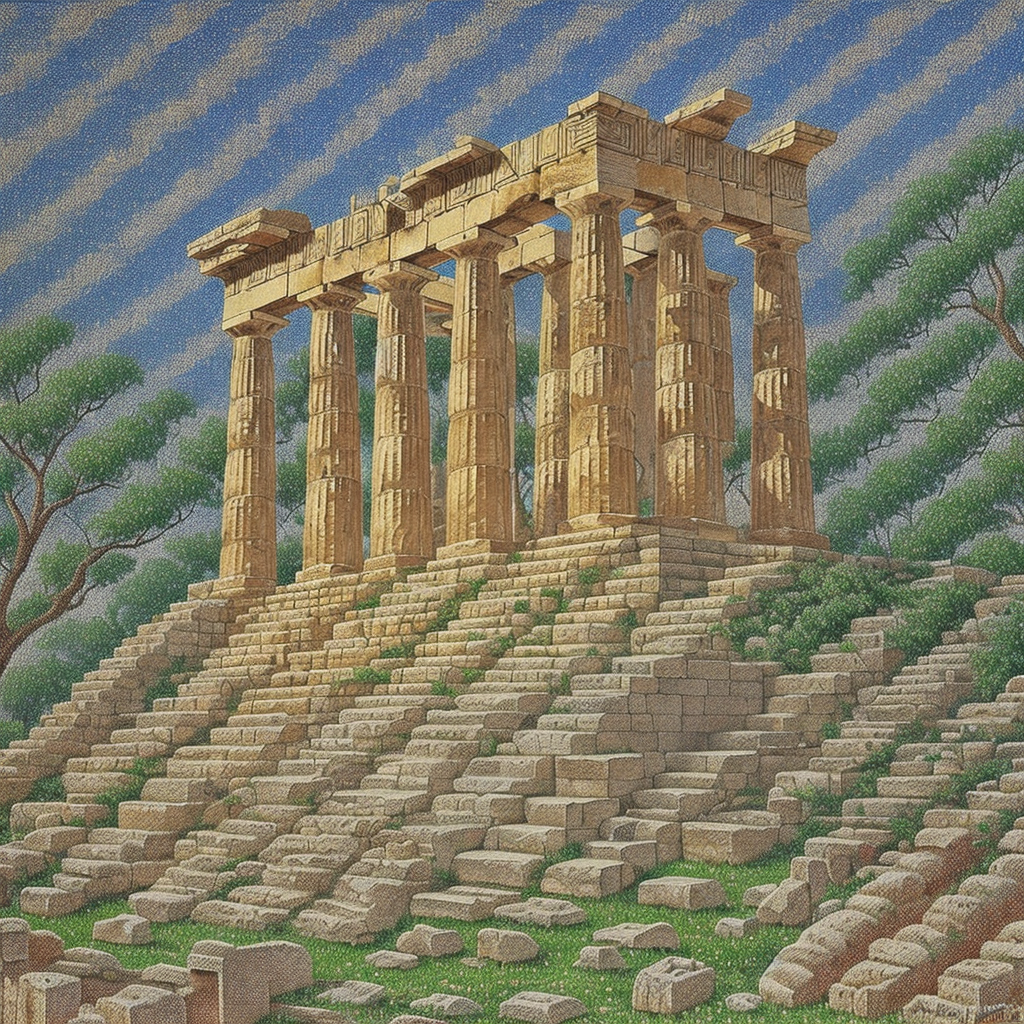
\includegraphics[width=0.65\textwidth]{Task1/01_original.png}
    \caption{Исходное изображение}
    \label{fig:task1_original}
\end{figure}

Изображение можно рассматривать как дискретную двумерную функцию. В случае чёрно-белого изображения каждому пикселю соответствует одно значение яркости:
\[
X:\mathbb{Z}^2 \to \mathbb{R}.
\]
Для цветного изображения каждому пикселю соответствует уже набор значений цветовых каналов, поэтому его можно рассматривать как отображение
\[
X:\mathbb{Z}^2 \to \mathbb{R}^3.
\]
В этом случае преобразование Фурье фактически применяется отдельно к каждому цветовому каналу.

\subsection*{Переход к Фурье-образу изображения}

Перед вычислением Фурье-образа изображение было приведено к вещественному типу, а значения яркости были нормированы делением на $255$. После этого было применено двумерное дискретное преобразование Фурье.

Для двумерного дискретного изображения прямое преобразование Фурье записывается в виде
\[
\widehat{X}(k_1,k_2)
=
\sum_{n_1=0}^{N_1-1}
\sum_{n_2=0}^{N_2-1}
X(n_1,n_2)
e^{-2\pi i\left(
\frac{n_1k_1}{N_1}
+
\frac{n_2k_2}{N_2}
\right)}.
\]

Здесь индексы $n_1,n_2$ задают координаты пикселя исходного изображения, а $k_1,k_2$ задают координаты в частотной области. Поэтому двумерный Фурье-образ показывает, какие пространственные частоты присутствуют в изображении по горизонтальному и вертикальному направлениям.

После вычисления Фурье-образ был сдвинут так, чтобы нулевая частота находилась в центре изображения. Это удобно для анализа: центральная область отвечает за низкие частоты, то есть за плавные изменения яркости и основную структуру изображения, а удалённые от центра области соответствуют более высоким частотам.

Так как значения модуля Фурье-образа могут сильно отличаться по масштабу, для отображения использовался логарифм модуля:
\[
\log(1 + |\widehat{X}|).
\]
Прибавление единицы необходимо для того, чтобы избежать логарифмирования нуля, а сам логарифм позволяет сделать видимыми не только самые большие, но и более слабые частотные компоненты.

\begin{figure}[H]
    \centering
    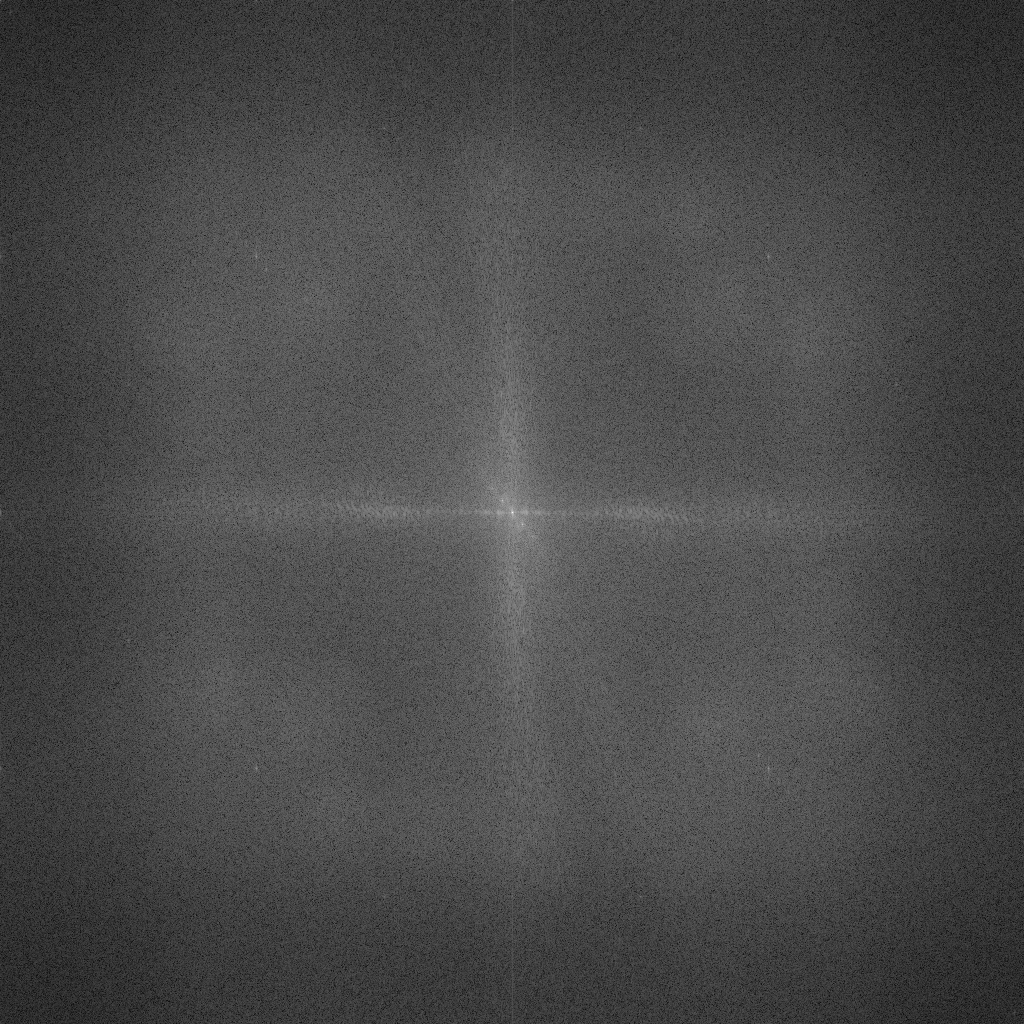
\includegraphics[width=0.65\textwidth]{Task1/02_fourier_log_module.png}
    \caption{Логарифм модуля Фурье-образа исходного изображения}
    \label{fig:task1_fourier}
\end{figure}

Для более удобного анализа был также построен приближенный вариант Фурье-образа.

\begin{figure}[H]
    \centering
    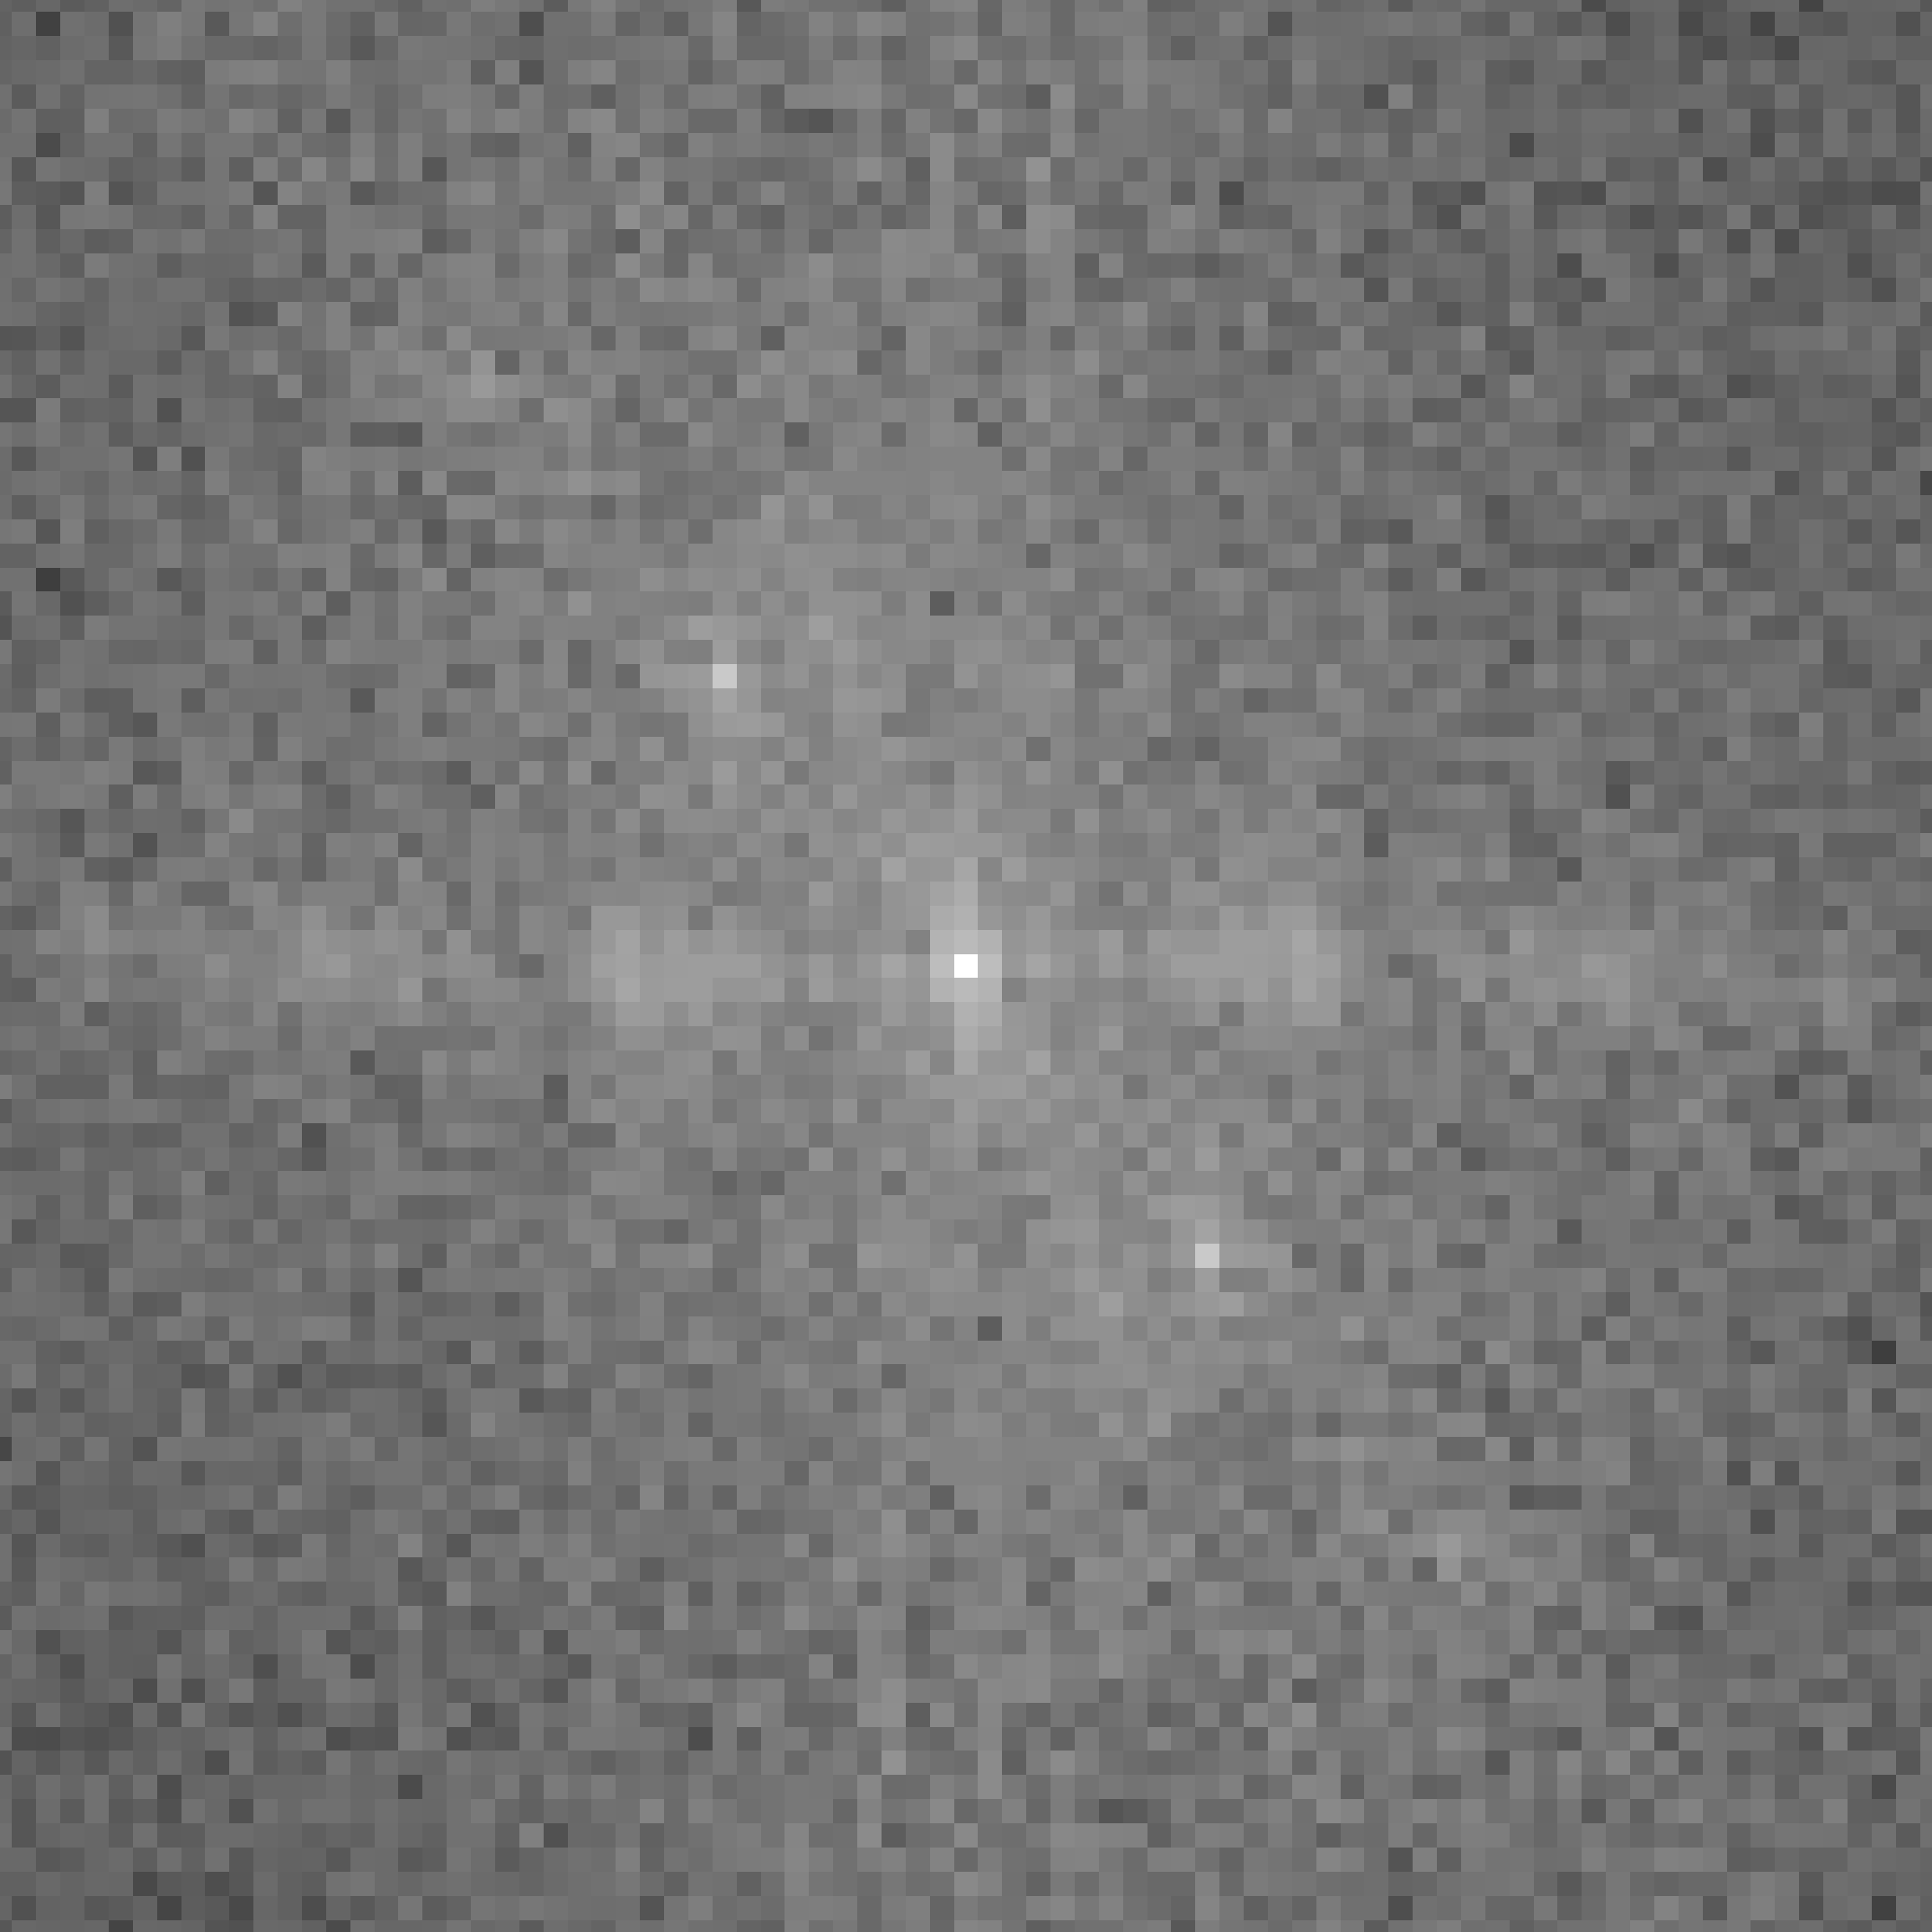
\includegraphics[width=0.65\textwidth]{Task1/02_fourier_log_module_zoom.png}
    \caption{Приближенный вид логарифма модуля Фурье-образа исходного изображения}
    \label{fig:task1_fourier_zoom}
\end{figure}

На Фурье-образе периодическая составляющая проявляется в виде отдельных ярких пиков. Это связано с тем, что регулярная повторяющаяся структура на исходной картинке соответствует отдельным выраженным гармоникам в частотной области. Именно поэтому частотная область удобна для удаления таких искажений: вместо работы со всей картинкой можно воздействовать только на небольшие области спектра.

\subsection*{Выделение лишних гармоник}

На следующем этапе на логарифме модуля Фурье-образа были выделены пики, которые соответствуют лишним гармоникам. Они расположены вне центральной низкочастотной области, поэтому их подавление не должно полностью разрушить основное содержание изображения.

В данной работе были выбраны следующие точки Фурье-образа:
\[
(502,\;500), \qquad (522,\;524).
\]
Они соответствуют частотным компонентам, связанным с периодическим искажением исходного изображения.


\begin{figure}[H]
    \centering
    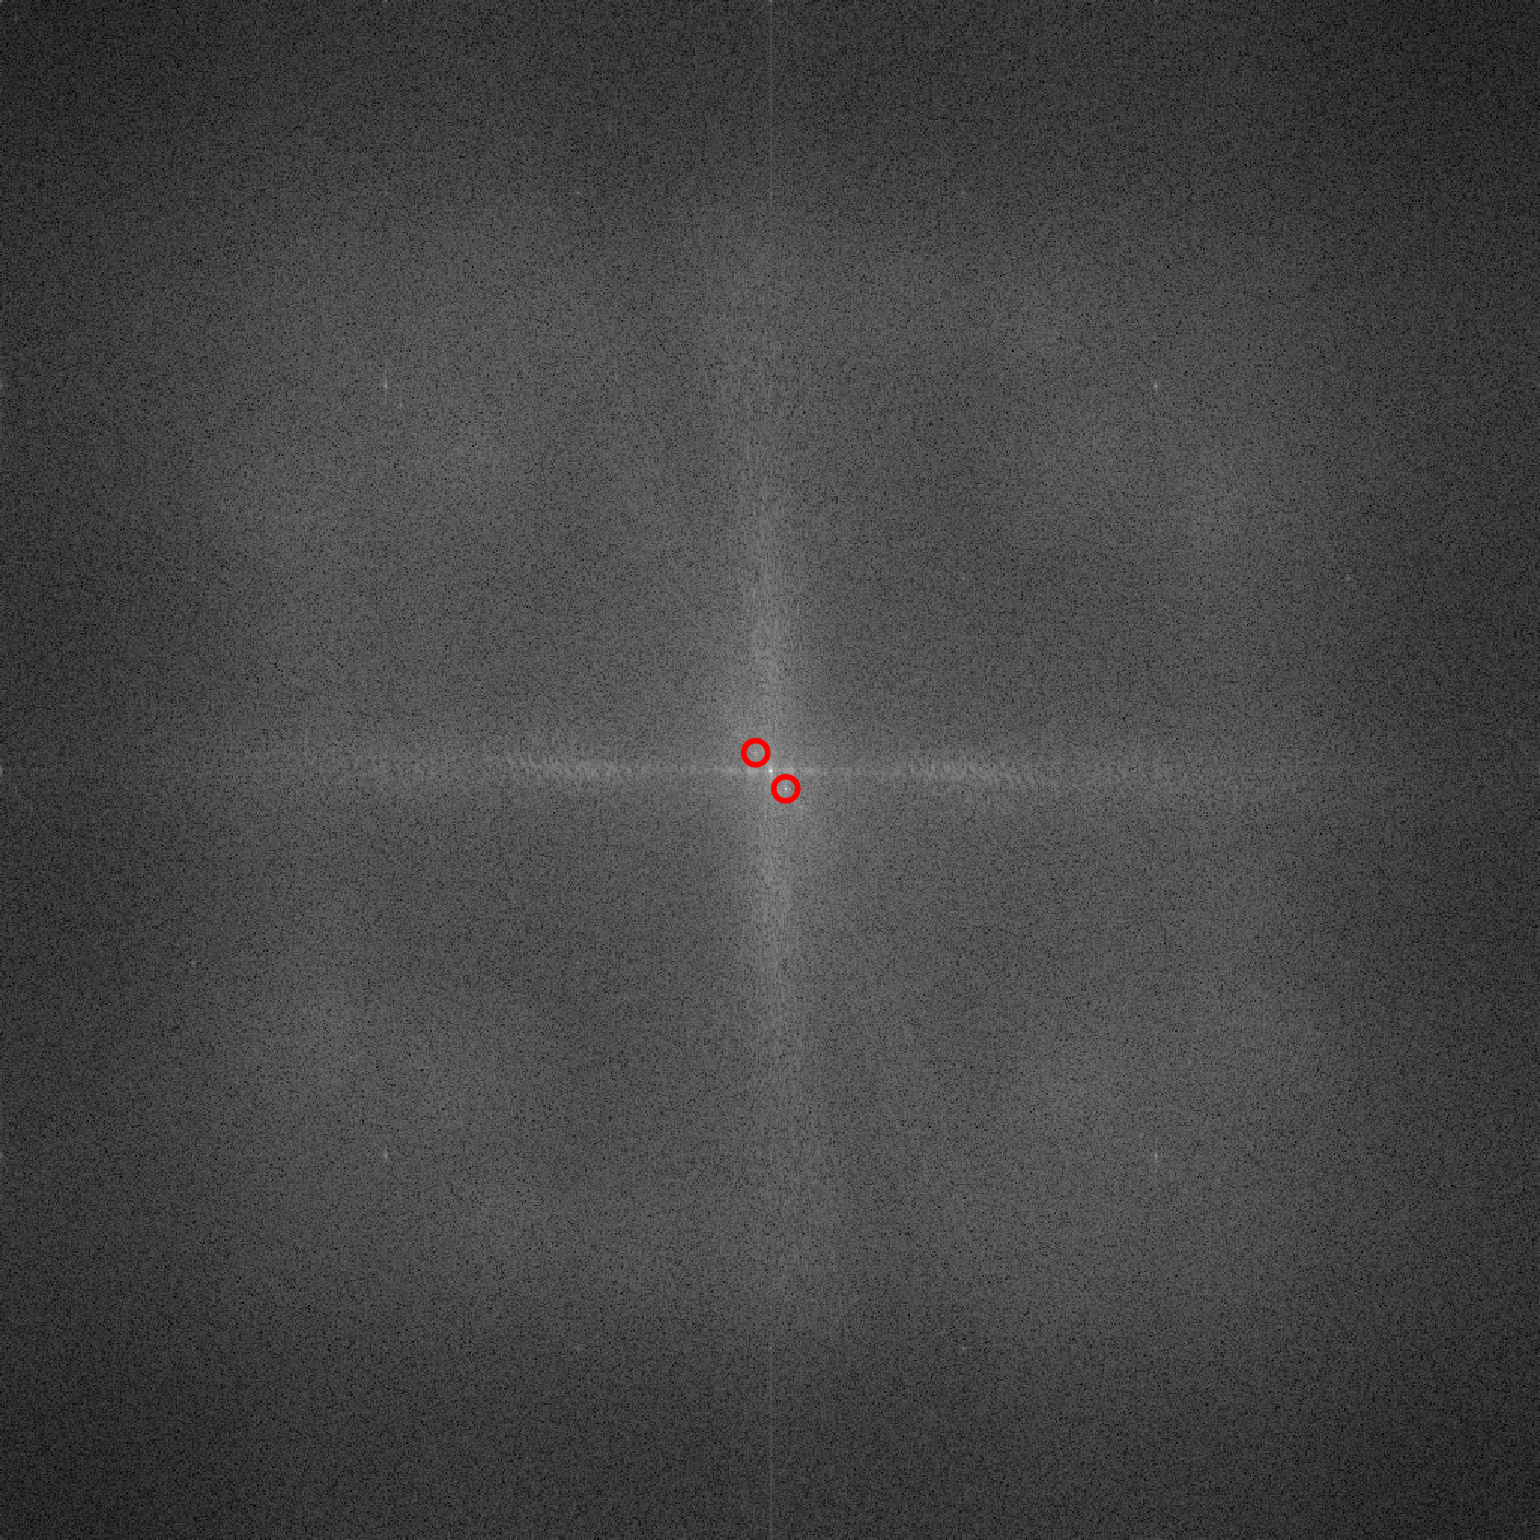
\includegraphics[width=0.65\textwidth]{Task1/03_fourier_log_module_with_marked_peaks.png}
    \caption{Фурье-образ с отмеченными пиками, соответствующими лишним гармоникам}
    \label{fig:task1_marked}
\end{figure}

\begin{figure}[H]
    \centering
    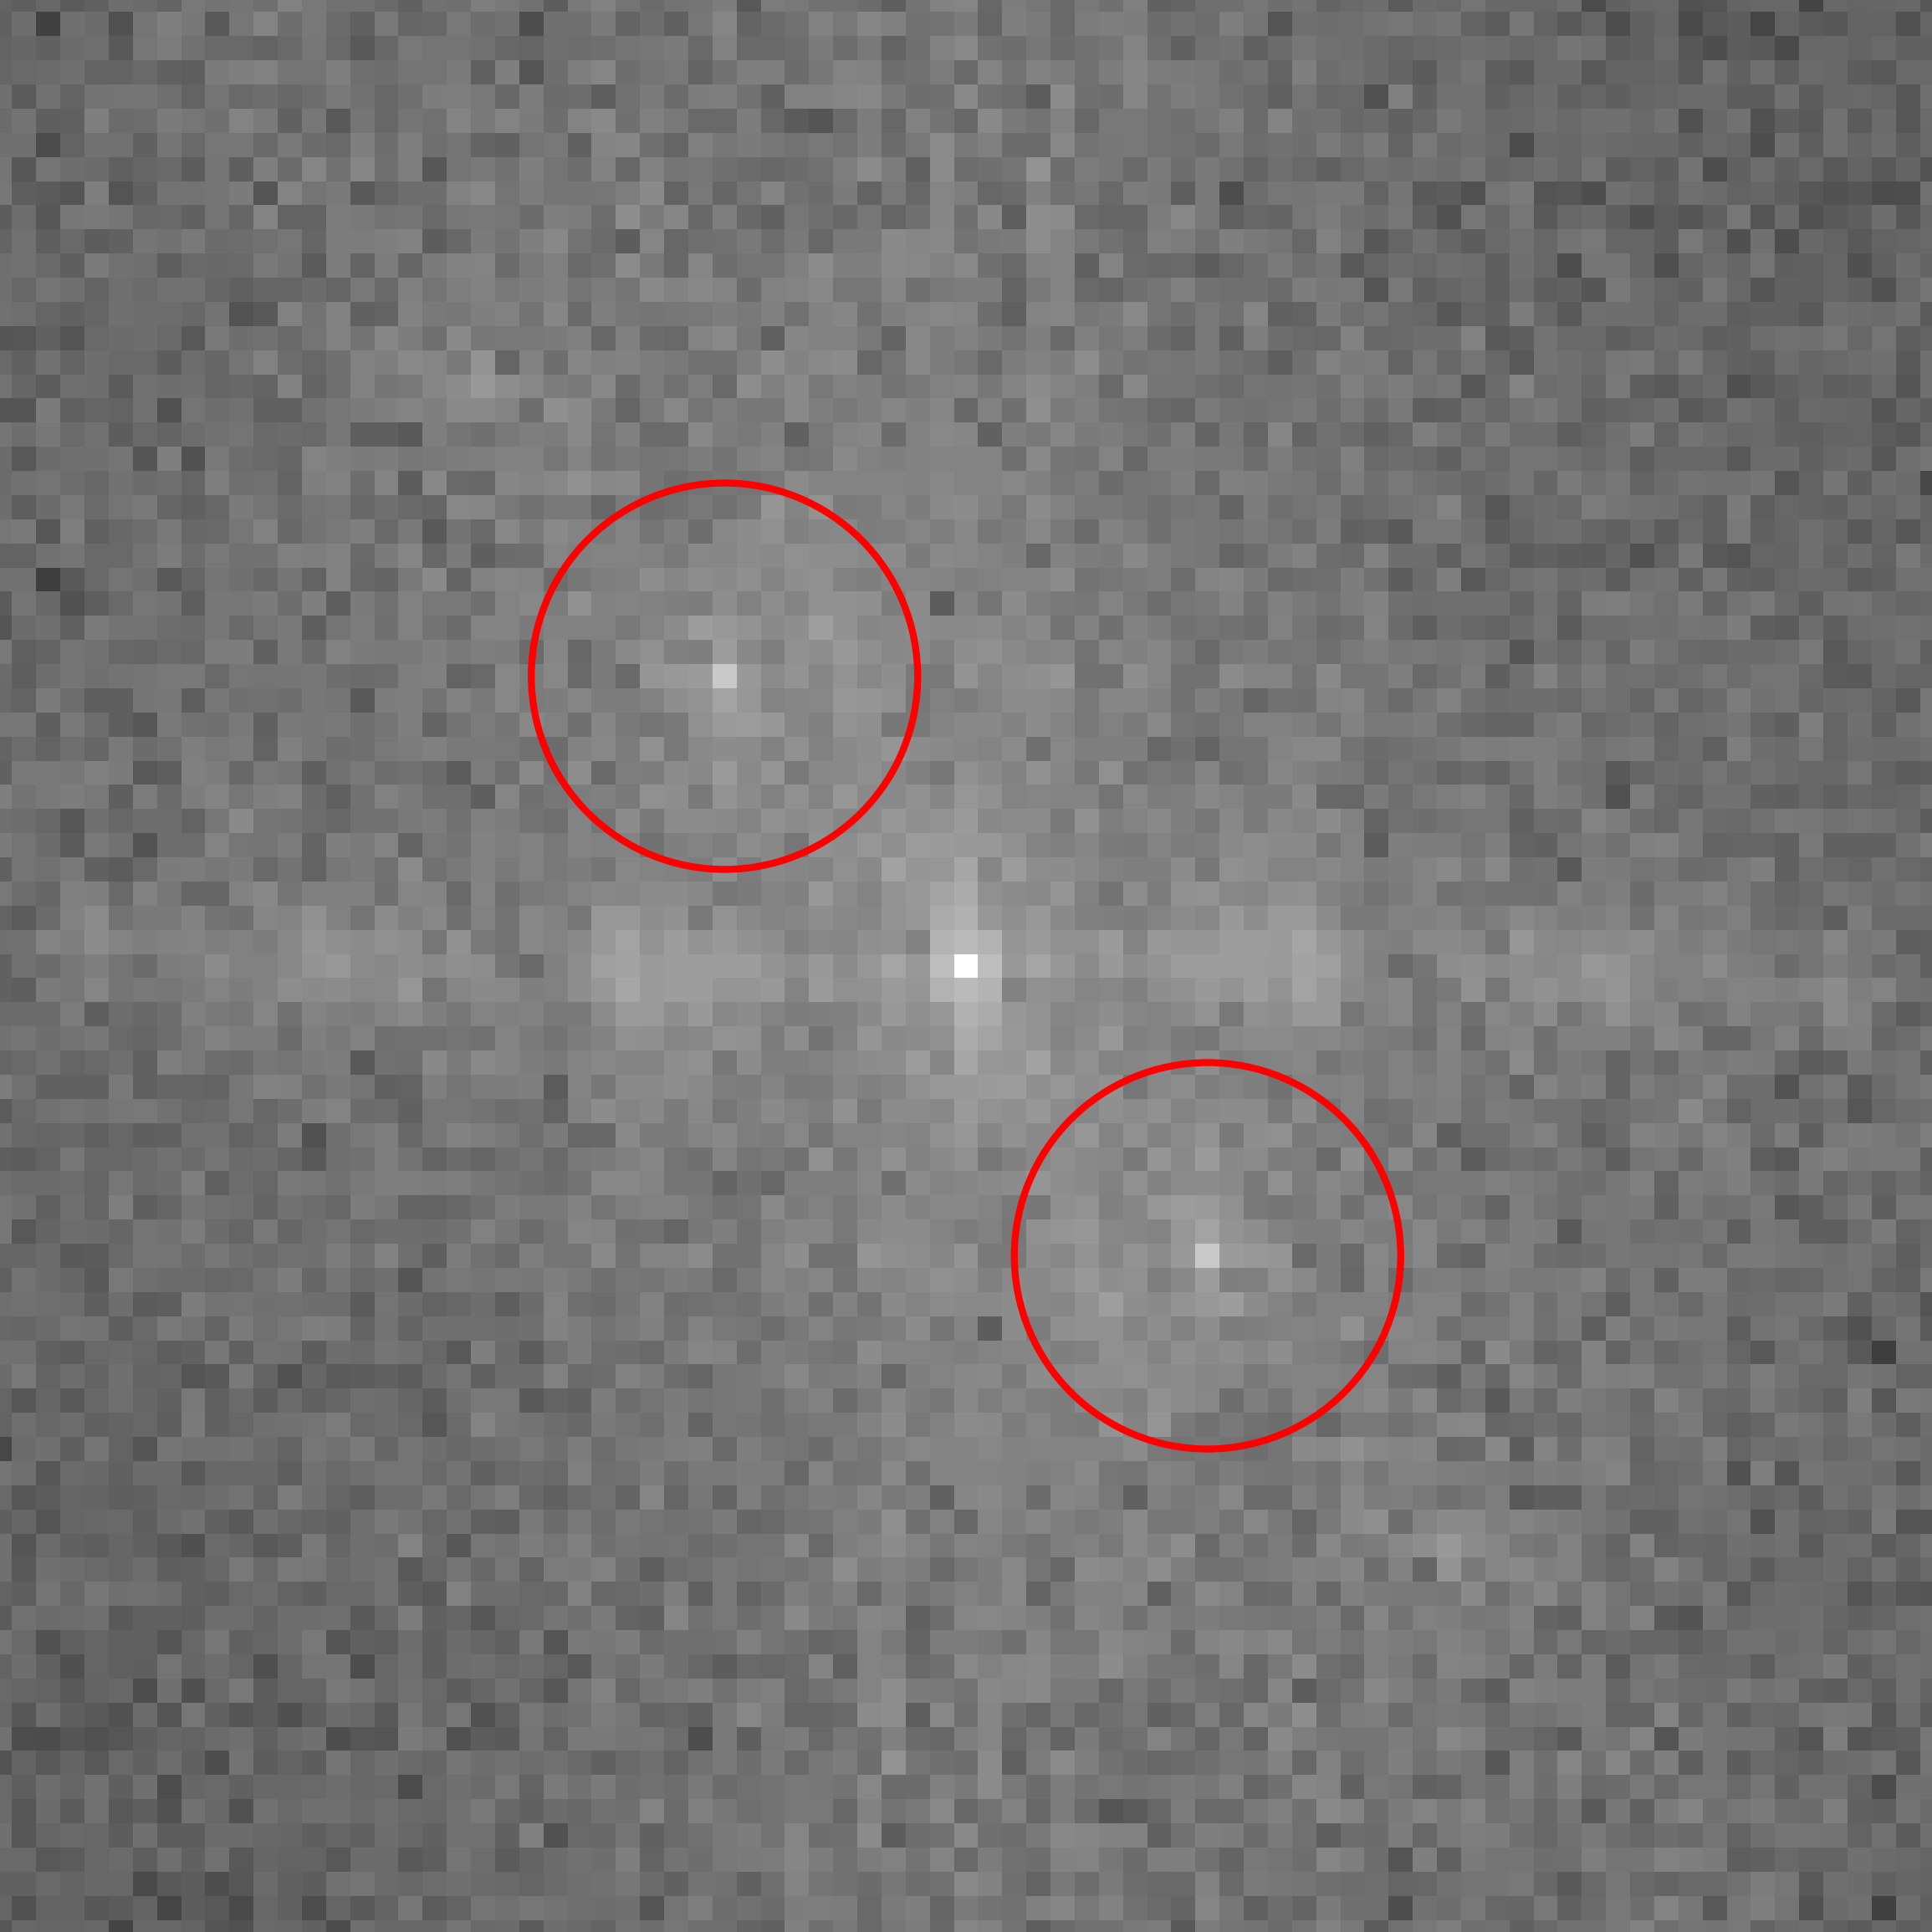
\includegraphics[width=0.65\textwidth]{Task1/03_fourier_log_module_with_marked_peaks_zoom.png}
    \caption{Приближенный вид Фурье-образа с отмеченными пиками}
    \label{fig:task1_marked_zoom}
\end{figure}

Важно, что подавлялась не только одна точка, а некоторая её окрестность. Это связано с тем, что периодическое искажение на практике редко сосредоточено строго в одном пикселе спектра. Обычно оно занимает небольшую локальную область вокруг яркого пика. Поэтому для фильтрации была выбрана окрестность вокруг найденных точек, а значения внутри неё заменялись усреднёнными значениями соседних элементов.

\subsection*{Подавление пиков и восстановление изображения}

После сглаживания выбранных областей был получен изменённый Фурье-образ. Его логарифм модуля имеет слудающий вид:

\begin{figure}[H]
    \centering
    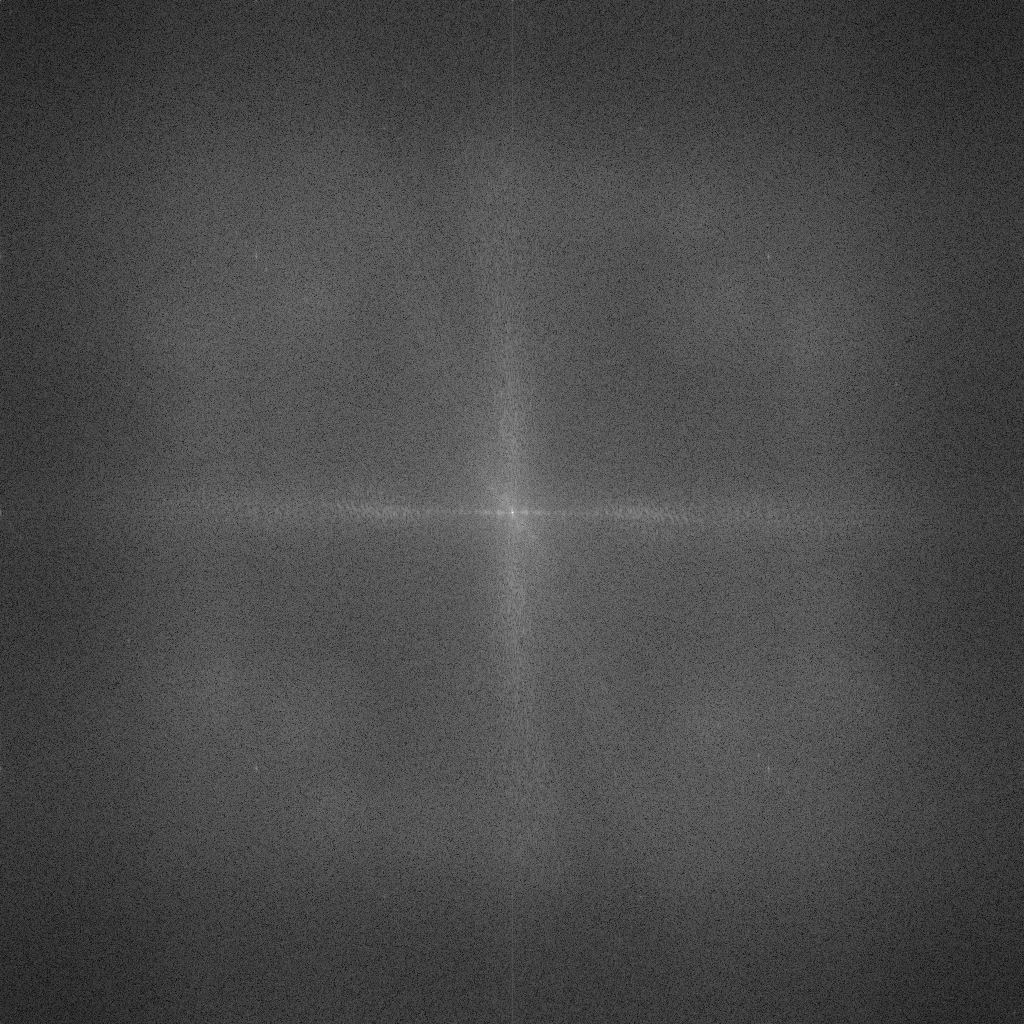
\includegraphics[width=0.65\textwidth]{Task1/04_fourier_log_module_filtered.png}
    \caption{Логарифм модуля Фурье-образа после подавления выбранных пиков}
    \label{fig:task1_filtered_spectrum}
\end{figure}

\begin{figure}[H]
    \centering
    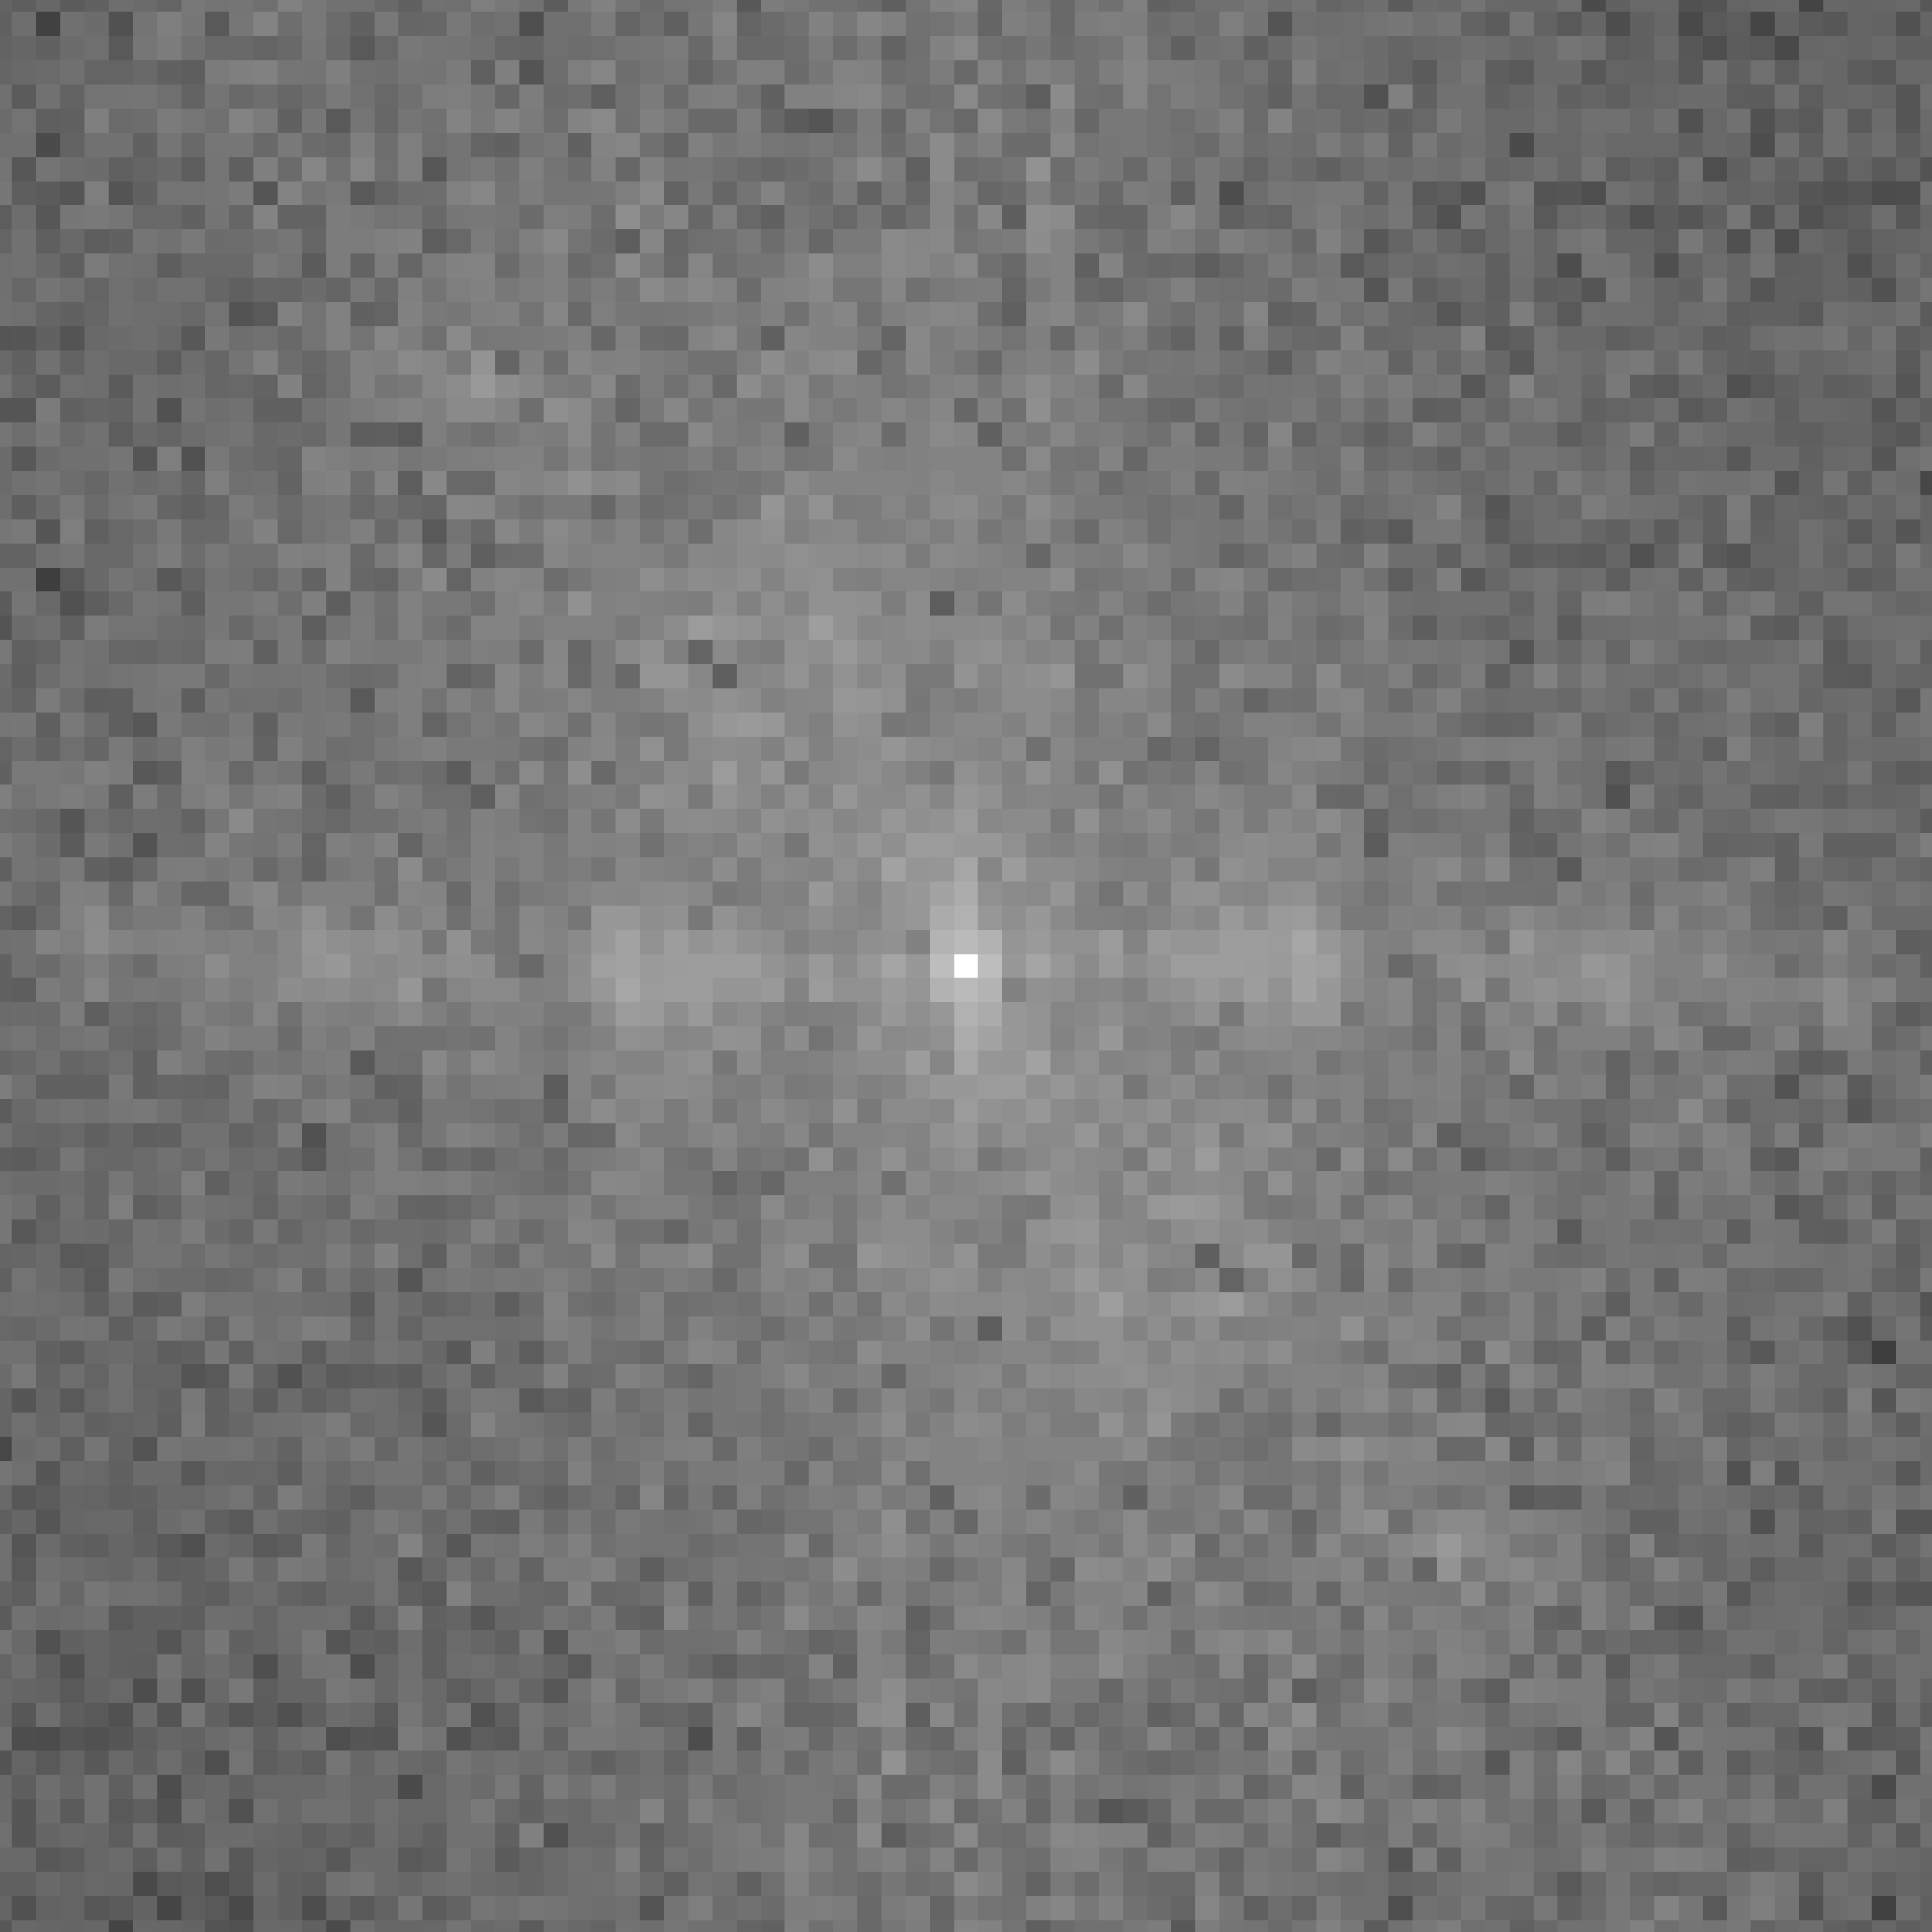
\includegraphics[width=0.65\textwidth]{Task1/04_fourier_log_module_filtered_zoom.png}
    \caption{Приближенный вид Фурье-образа после подавления выбранных пиков}
    \label{fig:task1_filtered_spectrum_zoom}
\end{figure}

После редактирования спектра было выполнено обратное двумерное преобразование Фурье:
\[
X(n_1,n_2)
=
\frac{1}{N_1N_2}
\sum_{k_1=0}^{N_1-1}
\sum_{k_2=0}^{N_2-1}
\widehat{X}(k_1,k_2)
e^{2\pi i\left(
\frac{n_1k_1}{N_1}
+
\frac{n_2k_2}{N_2}
\right)}.
\]

Смысл этого шага состоит в возвращении из частотной области обратно в пространственную область изображения. Если в Фурье-образе были подавлены частоты, отвечающие за периодическую помеху, то после обратного преобразования соответствующая периодическая структура должна стать менее выраженной.

Полученное изображение после фильтрации представлено на рис.~\ref{fig:task1_filtered_image}.

\begin{figure}[H]
    \centering
    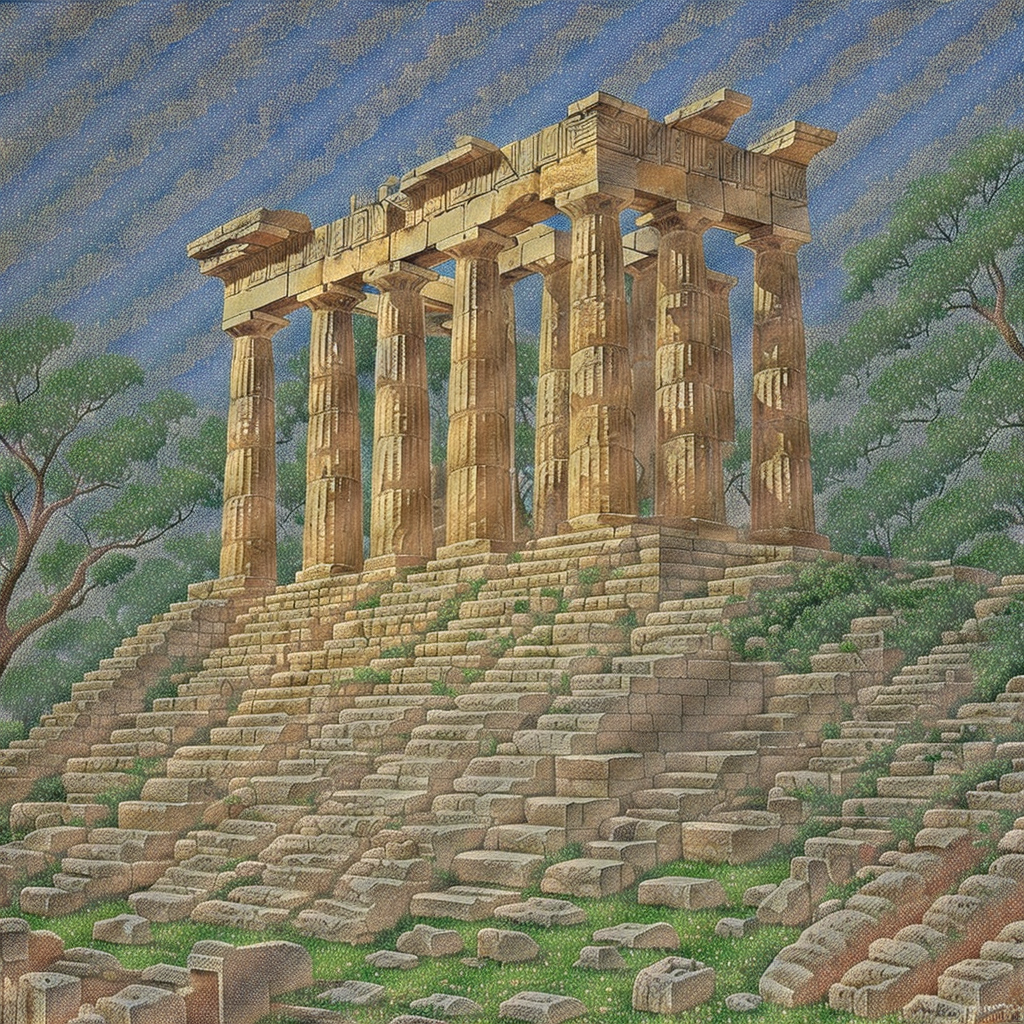
\includegraphics[width=0.65\textwidth]{Task1/05_filtered_image.png}
    \caption{Изображение после частотной фильтрации}
    \label{fig:task1_filtered_image}
\end{figure}

Для наглядного сравнения исходное и обработанное изображения расположены рядом на рис.~\ref{fig:task1_compare}.

\begin{figure}[H]
    \centering
    \subfloat[Исходное изображение]{
        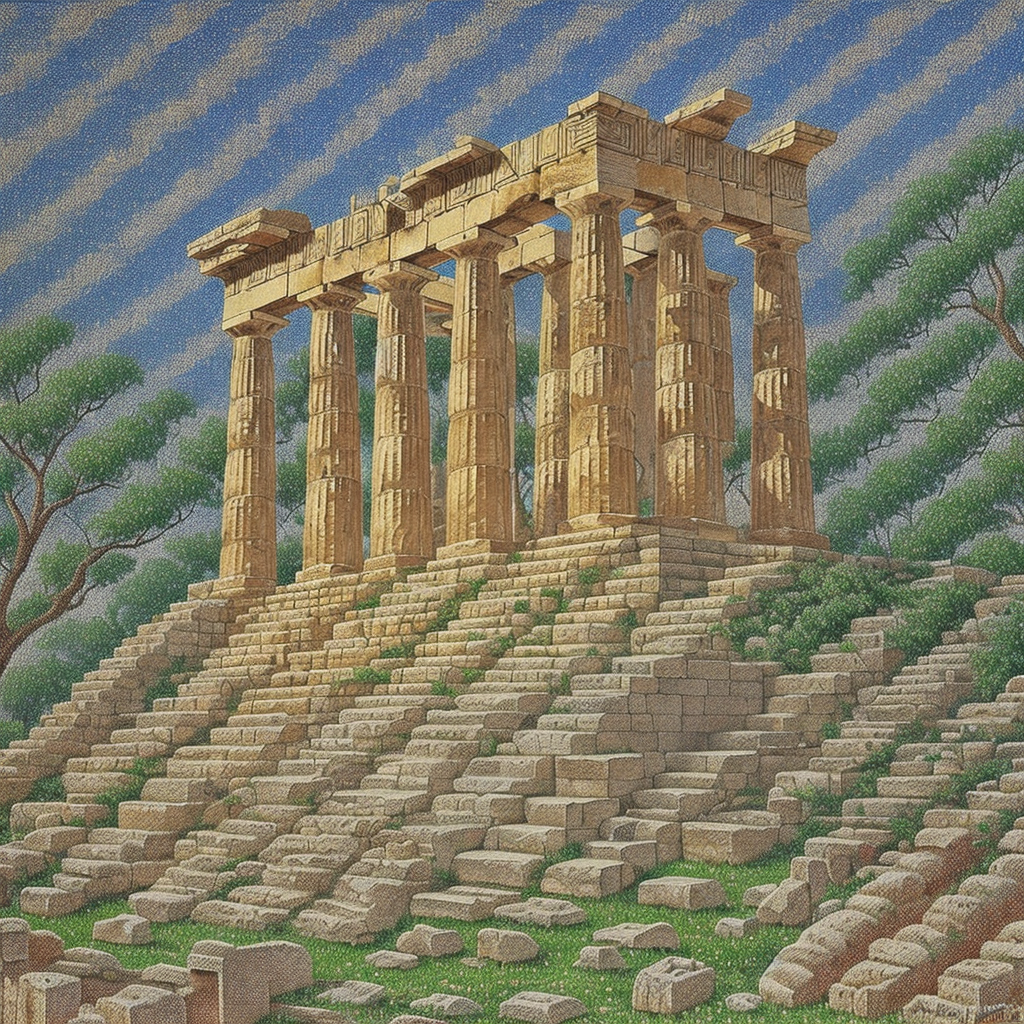
\includegraphics[width=0.45\textwidth]{Task1/01_original.png}
    }
    \hfill
    \subfloat[После фильтрации]{
        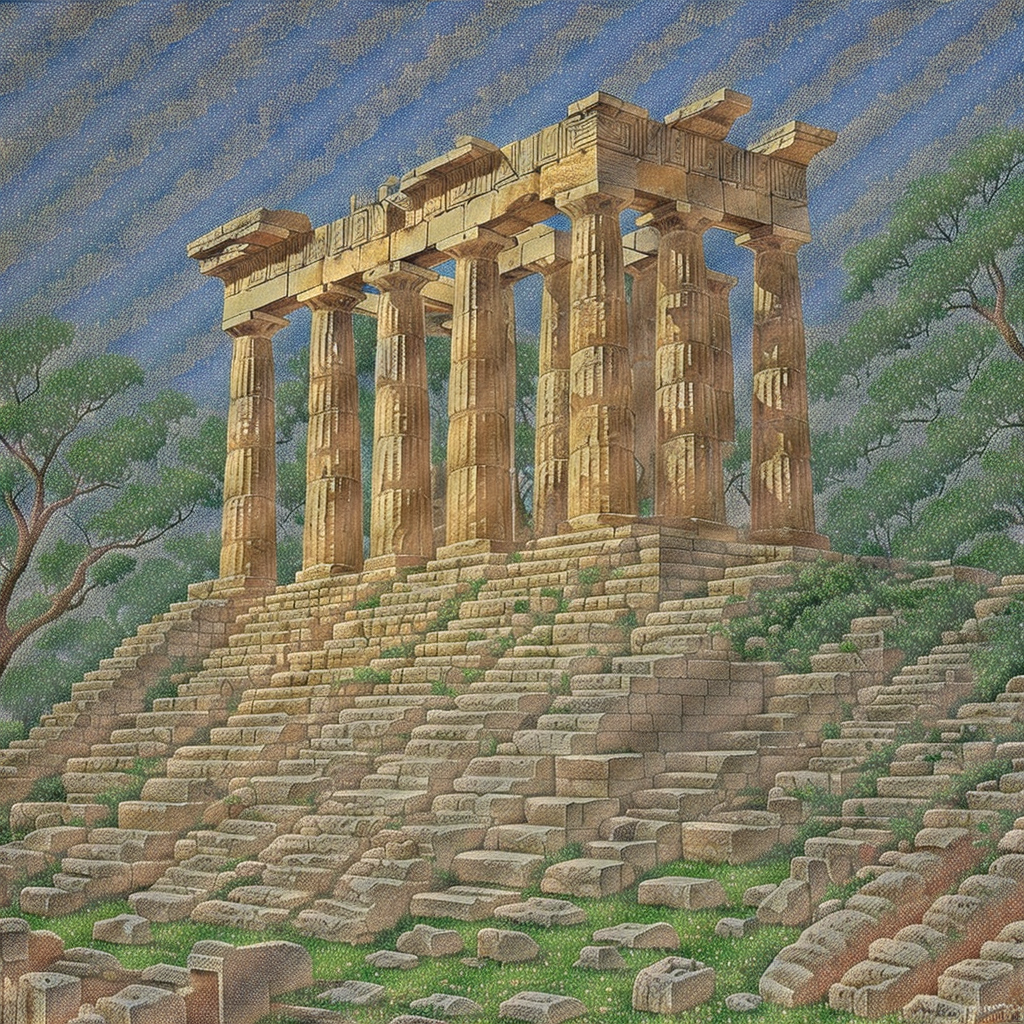
\includegraphics[width=0.45\textwidth]{Task1/05_filtered_image.png}
    }
    \caption{Сравнение исходного и отфильтрованного изображений}
    \label{fig:task1_compare}
\end{figure}

\subsection*{Анализ результата}

После подавления выбранных пиков периодическая составляющая на изображении стала менее выраженной. Основное содержание изображения при этом сохранилось, так как редактирование выполнялось локально и не затрагивало центральную низкочастотную область спектра.

Выбранные пики соответствовали лишним гармоникам, связанным с периодическим искажением. Их сглаживание позволило уменьшить вклад этих частот в восстановленное изображение.

Таким образом, обработка Фурье-образа позволила ослабить регулярную помеху без сильного искажения исходной структуры изображения.

\subsection*{Вывод по заданию}

В ходе выполнения задания было выполнено двумерное преобразование Фурье изображения с периодической составляющей. После построения логарифма модуля Фурье-образа были найдены ярко выраженные пики, соответствующие лишним гармоникам.

Для подавления периодического искажения были сглажены окрестности выбранных точек спектра:
\[
(502,\;500), \qquad (522,\;524).
\]
После обратного преобразования Фурье было получено изображение, на котором периодическая помеха стала менее выраженной.

Таким образом, было показано, что периодические искажения удобно удалять в частотной области: в исходном изображении они распределены по всей картинке, а в Фурье-образе проявляются как локальные пики. Их подавление позволяет ослабить нежелательную периодичность, сохранив при этом основную структуру изображения.


\section*{Задание 2. Исследование свёртки}

\subsection*{Загрузка изображения}

Сначала мы выбрали пиксель арт размером 32 на 32 пикселя с грустной жабой, поскольку она прекрасно отражает моральное состояние студентов в конце сессии. Далее по заданию (и чтобы предать картинке еще более грустный вид) перевели ее в черно-белый формат с помощью команды \texttt{convert('L')} в Python. Ниже оригинал и ее черно-белый аналог:

\begin{figure}[H]
    \centering
    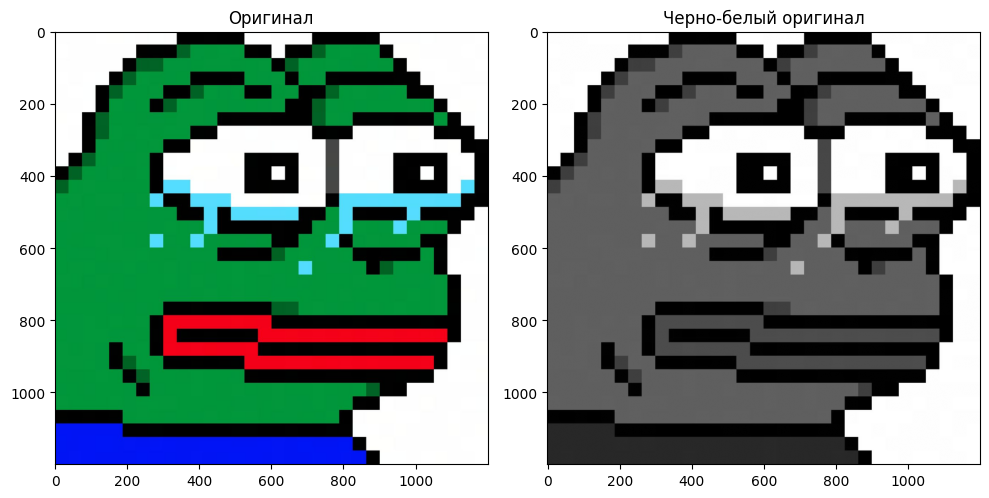
\includegraphics[width=1.0\textwidth]{2.1 Оригинал и чб.png}
    \caption{Результат пункта №1}
    \label{fig:original}
\end{figure}

\subsection*{Исследование ядер свёртки}

Далее мы решили объединить пункты и разбить их по 'буквам'. Для каждого случая продемонстрируем результаты формул и обработки картинок. Для трёх показательных нечётных значений $N \geq 3$ (мы выбрали $N = [3, 5, 7]$) определили четыре типа ядер. Начнем с ядер размытия двух типов!

\subsubsection*{а) Ядра размытия по Гауссу}

Для начала немного формул и теории. Ядро Гаусса вычисляется по формулам:
\begin{equation}
\sigma = \frac{N-1}{6}, \quad
A_{ij} = \exp\left(-\frac{(i - \frac{N+1}{2})^2 + (j - \frac{N+1}{2})^2}{2\sigma^2}\right), \quad
K_{\sigma} = \frac{A}{\sum_{i,j} A_{ij}}.
\end{equation}

\paragraph*{Размытие при $N = 3$}
\hfill\\[5pt]

Ядро Гаусса ($\sigma = 1/3$):
\begin{equation*}
K_{\sigma}^{(3)} = \begin{bmatrix}
0.0001 & 0.0106 & 0.0001 \\
0.0106 & 0.9570 & 0.0106 \\
0.0001 & 0.0106 & 0.0001
\end{bmatrix}
\end{equation*}

\begin{figure}[H]
    \centering
    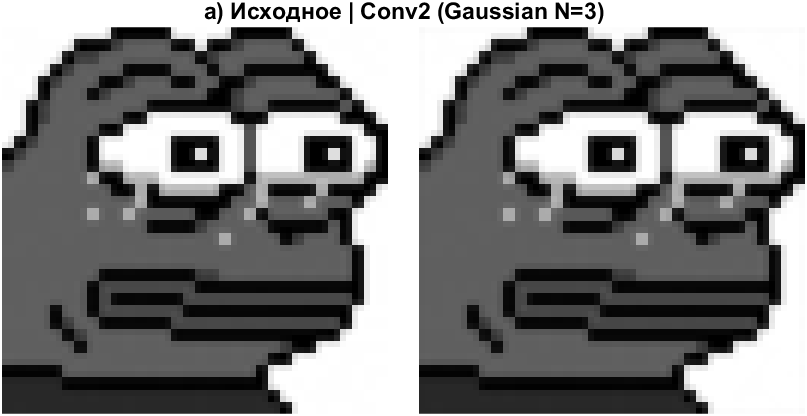
\includegraphics[width=0.8\textwidth]{a)/N=3/Orig_conv2.png}
    \caption{Слева - исходное чёрно-белое изображение, справа - результат свёртки изображения с гауссовым ядром при $N=3$.}
\end{figure}
При использовании гауссова ядра размера $3 \times 3$ эффект размытия выражен слабо. Изображение становится немного более сглаженным, однако основные контуры и детали сохраняются. Поскольку наибольший вес сосредоточен в центральной части ядра, размытие выглядит естественным и не приводит к резкому ухудшению качества изображения.


Для более глубокого понимания работы фильтров рассмотрим представление изображения в частотной области. Это позволяет анализировать не только пространственные изменения, но и распределение частотных компонент изображения.



\textbf{Дискретное преобразование Фурье (ДПФ)} переводит изображение из пространственной области в частотную:

\begin{equation}
F(u,v) = \sum_{x=0}^{h-1}\sum_{y=0}^{w-1} f(x,y) \cdot e^{-2\pi i(\frac{ux}{w} + \frac{vy}{h})},
\end{equation}

где $h$ и $w$ -- высота и ширина изображения.
\clearpage
\paragraph*{Спектр ядра}


Для анализа фильтра в частотной области был вычислен двумерный Фурье-образ ядра:
\[
H(u,v)=\mathcal{F}\{K_{\sigma}\}.
\]

На рисунке ниже представлен логарифм модуля спектра ядра:
\[
\log(1+|H(u,v)|).
\]

\begin{figure}[H]
    \centering
    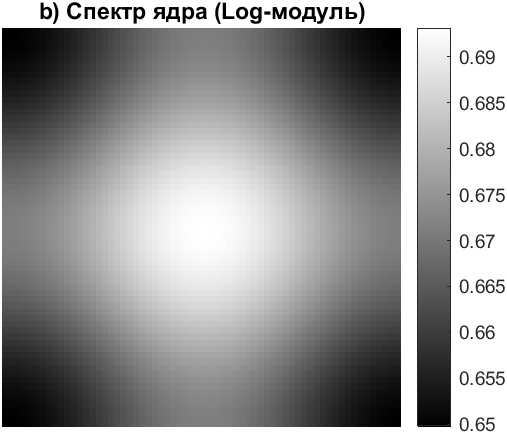
\includegraphics[width=0.48\textwidth]{a)/N=3/conv2_spektr.png}
    \caption{Логарифм модуля спектра гауссова ядра при $N=3$.}
\end{figure}
Центральная область спектра соответствует низким частотам и описывает общую структуру изображения.
Удалённые области спектра соответствуют высоким частотам и отвечают за границы, детали и шум.
Пики на спектре отражают доминирующие периодические структуры изображения.
Таким образом, фильтрация изображения может быть выполнена как в пространственной, так и в частотной области.
Частотное представление удобно тем, что операция свёртки заменяется простым поэлементным умножением спектров.
Из спектра видно, что гауссов фильтр усиливает низкие частоты и подавляет высокочастотные компоненты изображения. Именно поэтому изображение становится более размытым.




\paragraph*{Спектр фильтрованного изображения}
\

\textbf{Теорема о свёртке}

Согласно теореме о свёртке:
\[
\mathcal{F}\{f * g\} =
\mathcal{F}\{f\}\cdot
\mathcal{F}\{g\},
\]
где $f$ --- исходное изображение, а $g$ --- ядро фильтра.


Свёртка в пространственной области эквивалентна поэлементному умножению в частотной области:

\begin{equation}
f * g = \mathcal{F}^{-1}\{\mathcal{F}\{f\} \cdot \mathcal{F}\{g\}\}.
\end{equation}

\textbf{Дополнение нулями (Zero Padding)}: для избежания циклической свёртки размеры дополняются до $(h+k-1, w+l-1)$, где $k$ и $l$ -- высота и ширина ядра.

Сначала вычисляется Фурье-образ изображения и ядра, затем они перемножаются поэлементно. После этого выполняется обратное преобразование Фурье.

На рисунке ниже показан логарифм модуля спектра обработанного изображения:
\[
\log(1+|F(u,v)H(u,v)|).
\]

\begin{figure}[H]
    \centering
    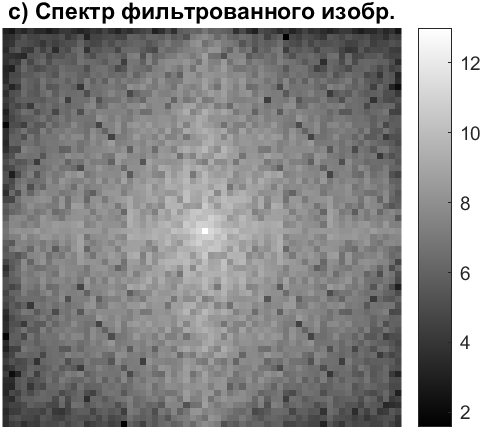
\includegraphics[width=0.48\textwidth]{a)/N=3/filt_spektr.png}
    \caption{Логарифм модуля спектра изображения после фильтрации гауссовым ядром.}
\end{figure}

После фильтрации высокочастотные детали становятся менее выраженными, что соответствует эффекту сглаживания изображения.

\paragraph*{Сравнение свёртки и преобразования Фурье}

Для проверки теоремы о свёртке обработка изображения была выполнена двумя способами:
\begin{enumerate}
    \item непосредственной свёрткой с помощью функции \texttt{conv2};
    \item через преобразование Фурье:
    \[
    y = \mathcal{F}^{-1}
    \left(
    \mathcal{F}(f)\cdot \mathcal{F}(g)
    \right).
    \]
\end{enumerate}

\begin{figure}[H]
    \centering
    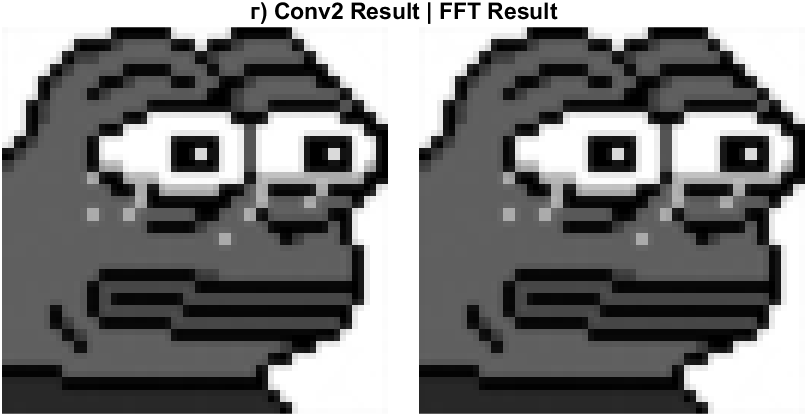
\includegraphics[width=0.8\textwidth]{a)/N=3/conv2_FFT.png}
    \caption{Сравнение результата свёртки и результата, полученного через преобразование Фурье.}
\end{figure}

Из рисунка видно, что результаты практически совпадают. Незначительные различия могут возникать из-за погрешностей округления и особенностей обработки границ изображения. Таким образом, экспериментально подтверждается теорема о свёртке: свёртка в пространственной области эквивалентна поэлементному умножению спектров в частотной области.

\paragraph*{Размытие при $N = 5$}
\hfill\\[5pt]

Ядро Гаусса ($\sigma = 2/3$):
\begin{equation*}
K_{\sigma}^{(5)} = \begin{bmatrix}
0.0000 & 0.0013 & 0.0040 & 0.0013 & 0.0000 \\
0.0013 & 0.0377 & 0.1162 & 0.0377 & 0.0013 \\
0.0040 & 0.1162 & 0.3579 & 0.1162 & 0.0040 \\
0.0013 & 0.0377 & 0.1162 & 0.0377 & 0.0013 \\
0.0000 & 0.0013 & 0.0040 & 0.0013 & 0.0000
\end{bmatrix}
\end{equation*}




\begin{figure}[H]
    \centering
    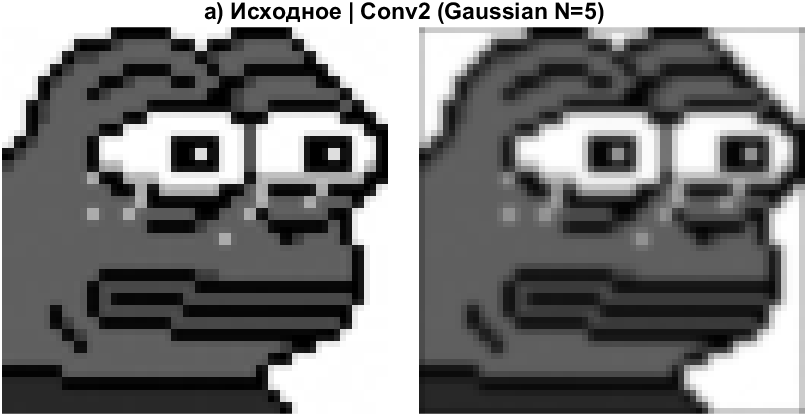
\includegraphics[width=0.8\textwidth]{a)/N=5/Orig_conv2.png}
    \caption{Слева - исходное чёрно-белое изображение, справа - результат свёртки изображения с гауссовым ядром при $N=5$.}
\end{figure}

По сравнению со случаем $N=3$ эффект размытия стал значительно заметнее. Изображение стало более сглаженным и слегка темнее, поскольку фильтр сильнее подавляет резкие перепады яркости и высокочастотные детали.

\paragraph*{Спектр ядра}

Для исследования фильтра в частотной области был вычислен двумерный Фурье-образ ядра:
\[
H(u,v)=\mathcal{F}\{K_{\sigma}\}.
\]

Ниже представлен логарифм модуля спектра ядра:
\[
\log(1+|H(u,v)|).
\]

\begin{figure}[H]
    \centering
    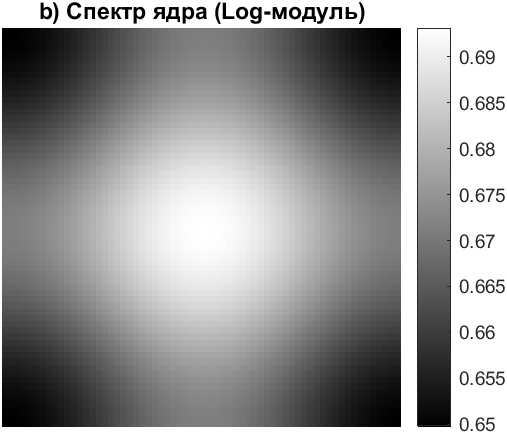
\includegraphics[width=0.48\textwidth]{a)/N=3/conv2_spektr.png}
    \caption{Логарифм модуля спектра гауссова ядра при $N=5$.}
\end{figure}

Спектр показывает, что при увеличении размера ядра фильтр ещё сильнее подавляет высокочастотные компоненты изображения. Низкие частоты сохраняются, а детали и резкие границы становятся менее выраженными.

\paragraph*{Спектр фильтрованного изображения}

После поэлементного перемножения спектра изображения и спектра ядра было выполнено обратное преобразование Фурье:
\[
y =
\mathcal{F}^{-1}
\left(
\mathcal{F}(f)\cdot
\mathcal{F}(g)
\right).
\]

На рисунке ниже представлен спектр фильтрованного изображения:

\begin{figure}[H]
    \centering
    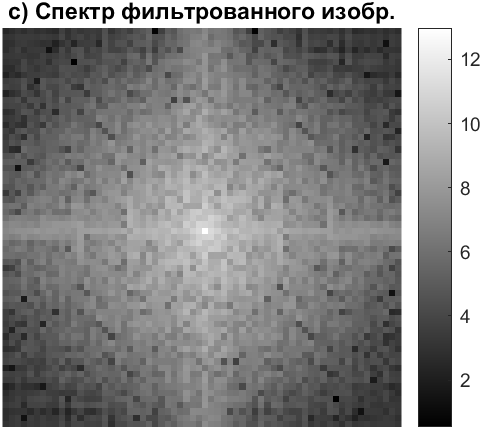
\includegraphics[width=0.48\textwidth]{a)/N=5/filt_spektr.png}
    \caption{Логарифм модуля спектра изображения после фильтрации гауссовым ядром при $N=5$.}
\end{figure}


\paragraph*{Сравнение свёртки и преобразования Фурье}

Для проверки теоремы о свёртке были сравнены результаты:
\begin{enumerate}
    \item свёртки изображения с помощью функции \texttt{conv2};
    \item фильтрации через преобразование Фурье.
\end{enumerate}

\begin{figure}[H]
    \centering
    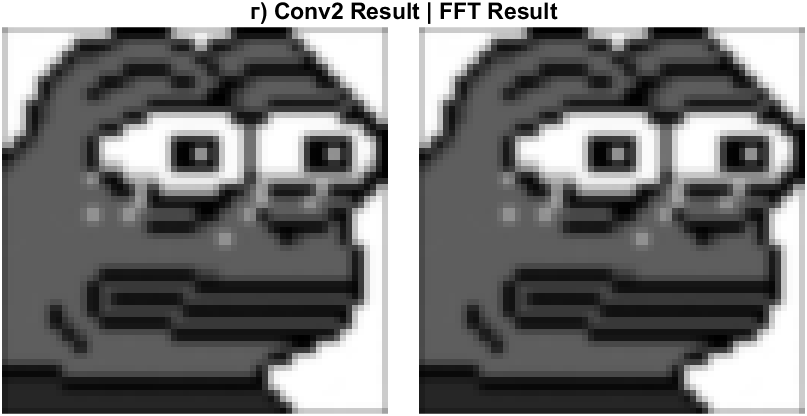
\includegraphics[width=0.8\textwidth]{a)/N=5/conv2_FFT.png}
    \caption{Сравнение результатов свёртки и обработки через преобразование Фурье при $N=5$.}
\end{figure}

\paragraph*{Размытие при $N = 7$}
\hfill\\[5pt]

Ядро Гаусса ($\sigma = 1$):
\begin{equation*}
K_{\sigma}^{(7)} = \begin{bmatrix}
0.0000 & 0.0002 & 0.0011 & 0.0018 & 0.0011 & 0.0002 & 0.0000 \\
0.0002 & 0.0029 & 0.0131 & 0.0216 & 0.0131 & 0.0029 & 0.0002 \\
0.0011 & 0.0131 & 0.0586 & 0.0966 & 0.0586 & 0.0131 & 0.0011 \\
0.0018 & 0.0216 & 0.0966 & 0.1592 & 0.0966 & 0.0216 & 0.0018 \\
0.0011 & 0.0131 & 0.0586 & 0.0966 & 0.0586 & 0.0131 & 0.0011 \\
0.0002 & 0.0029 & 0.0131 & 0.0216 & 0.0131 & 0.0029 & 0.0002 \\
0.0000 & 0.0002 & 0.0011 & 0.0018 & 0.0011 & 0.0002 & 0.0000
\end{bmatrix}
\end{equation*}


\begin{figure}[H]
    \centering
    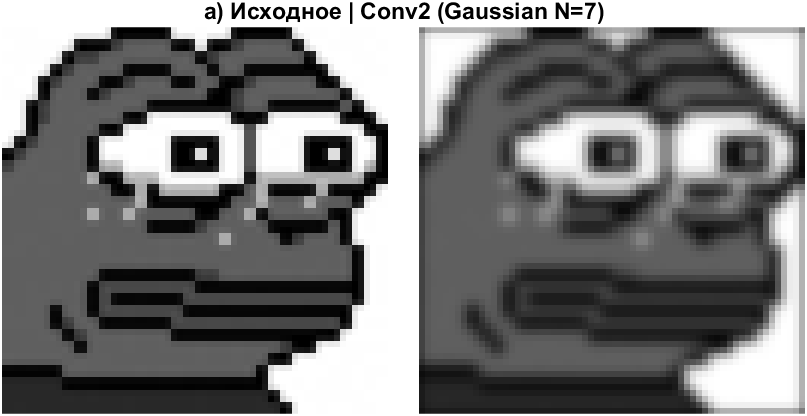
\includegraphics[width=0.8\textwidth]{a)/N=7/Orig_conv2.png}
    \caption{Слева - исходное чёрно-белое изображение, справа - результат свёртки изображения с гауссовым ядром при $N=7$.}
\end{figure}


При $N=7$ разница между ядрами стала явной: гауссово ядро даёт естественное размытие, которое будет не заметно, если вы не видели оригинала. А блочное - более 'мыльное', здесь размыты даже границы изображения!



\paragraph*{Спектр ядра}

Фурье-образ ядра:
\[
H(u,v)=\mathcal{F}\{K_{\sigma}\}.
\]

Логарифм модуля спектра ядра:

\begin{figure}[H]
    \centering
    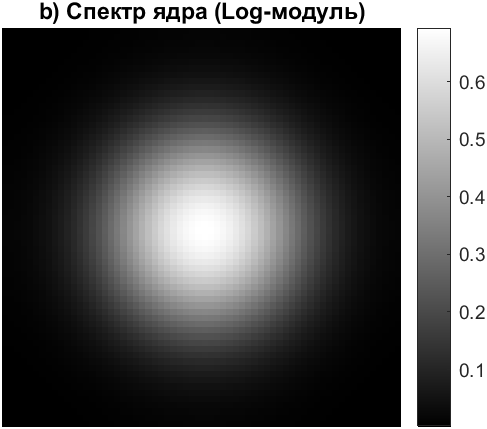
\includegraphics[width=0.48\textwidth]{a)/N=7/conv2_spektr.png}
    \caption{Логарифм модуля спектра гауссова ядра при $N=7$.}
\end{figure}

Из спектра видно ещё более сильное подавление высоких частот по сравнению с $N=3$ и $N=5$. Это объясняет более выраженное размытие изображения при увеличении размера ядра.

\paragraph*{Спектр фильтрованного изображения}

После применения фильтра в частотной области:
\[
y =
\mathcal{F}^{-1}
\left(
\mathcal{F}(f)\cdot
\mathcal{F}(g)
\right).
\]

Результат фильтрации в частотной области:

\begin{figure}[H]
    \centering
    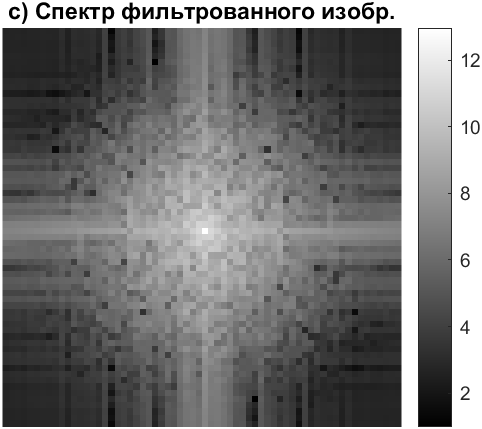
\includegraphics[width=0.48\textwidth]{a)/N=7/filt_spektr.png}
    \caption{Логарифм модуля спектра изображения после гауссова фильтра при $N=7$.}
\end{figure}

Высокочастотные компоненты практически полностью подавлены, что приводит к максимальному сглаживанию изображения среди всех рассмотренных случаев.

\paragraph*{Сравнение свёртки и преобразования Фурье}

\ 

Сравнение двух способов обработки:

\begin{enumerate}
    \item свёртка через \texttt{conv2};
    \item обработка через преобразование Фурье.
\end{enumerate}

\begin{figure}[H]
    \centering
    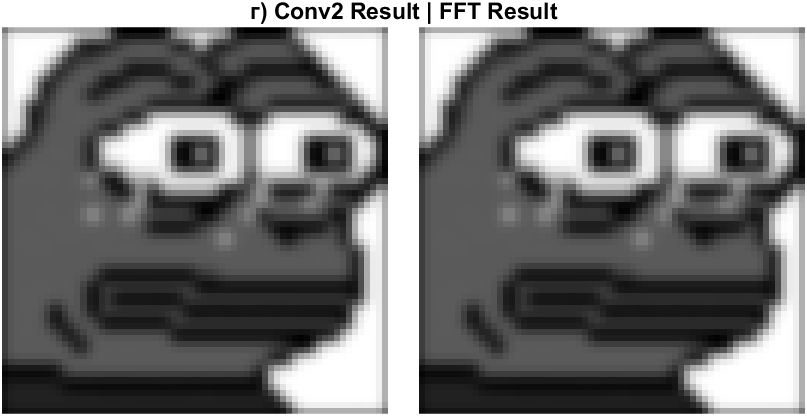
\includegraphics[width=0.8\textwidth]{a)/N=7/conv2_FFT.png}
    \caption{Сравнение результатов свёртки и обработки через преобразование Фурье при $N=7$.}
\end{figure}

Как и в предыдущих случаях, результаты двух методов практически совпадают, что подтверждает корректность численной реализации теоремы о свёртке. Отличия минимальны и обусловлены дискретизацией и округлением.

%===============================================
\subsubsection*{б) Ядра блочного размытия}

Для начала немного формул и теории. Ядро блочного размытия считается через равномерное усреднение:
\begin{equation}
A_{ij} = 1, \quad K_{\Box} = \frac{A}{\sum_{i,j} A_{ij}} = \frac{1}{N^2}\mathbf{1}_{N\times N}.
\end{equation}

\paragraph*{Размытие при $N = 3$}
\hfill\\[5pt]

Ядро блочного размытия:
\begin{equation*}
K_{\Box}^{(3)} = \frac{1}{9}\begin{bmatrix}
1 & 1 & 1 \\
1 & 1 & 1 \\
1 & 1 & 1
\end{bmatrix} = \begin{bmatrix}
0.1111 & 0.1111 & 0.1111 \\
0.1111 & 0.1111 & 0.1111 \\
0.1111 & 0.1111 & 0.1111
\end{bmatrix}
\end{equation*}


\paragraph*{Размытие при $N = 3$}

\begin{figure}[H]
    \centering
    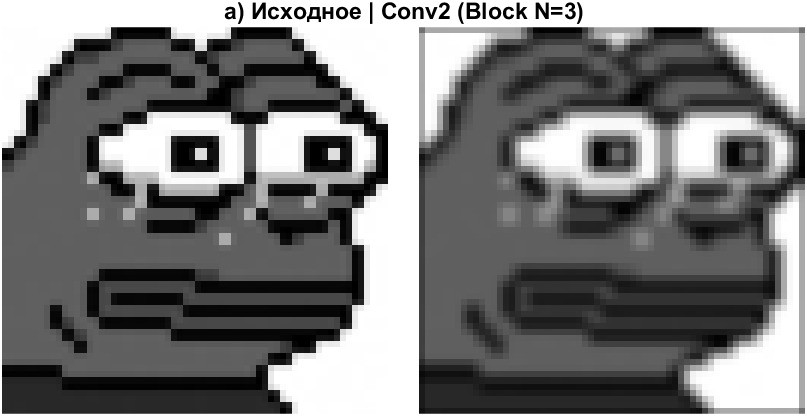
\includegraphics[width=0.8\textwidth]{б)/N=3/Orig_conv2.png}
    \caption{Слева - исходное чёрно-белое изображение, справа - результат свёртки с блочным ядром при $N=3$.}
\end{figure}

При использовании ядра блочного размытия размера $3 \times 3$ изображение становится более сглаженным за счёт равномерного усреднения соседних пикселей. В отличие от гауссова фильтра, размытие выглядит менее естественным: границы объектов становятся более размытыми, а мелкие детали начинают теряться.



\begin{figure}[H]
    \centering
    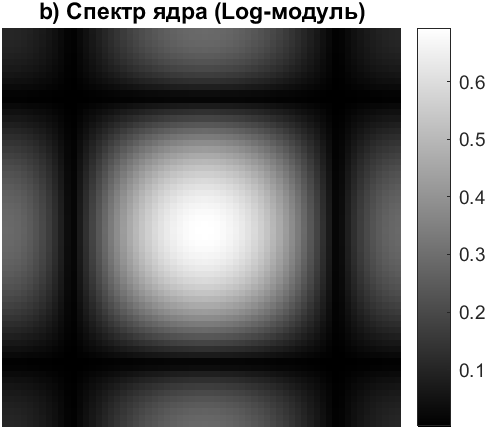
\includegraphics[width=0.8\textwidth]{б)/N=3/conv2_spektr.png}
    \caption{Спектр ядра блочного размытия при $N=3$.}
\end{figure}

\begin{figure}[H]
    \centering
    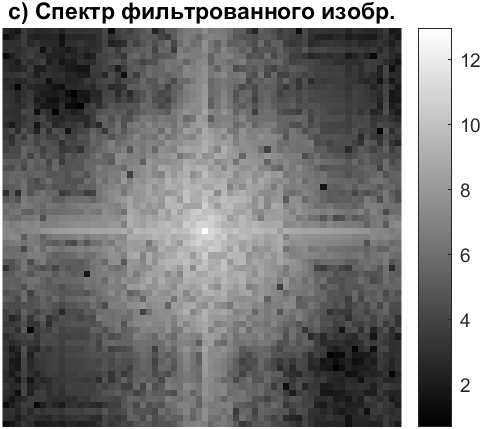
\includegraphics[width=0.8\textwidth]{б)/N=3/filt_spektr.png}
    \caption{Спектр фильтрованного изображения при $N=3$.}
\end{figure}

\begin{figure}[H]
    \centering
    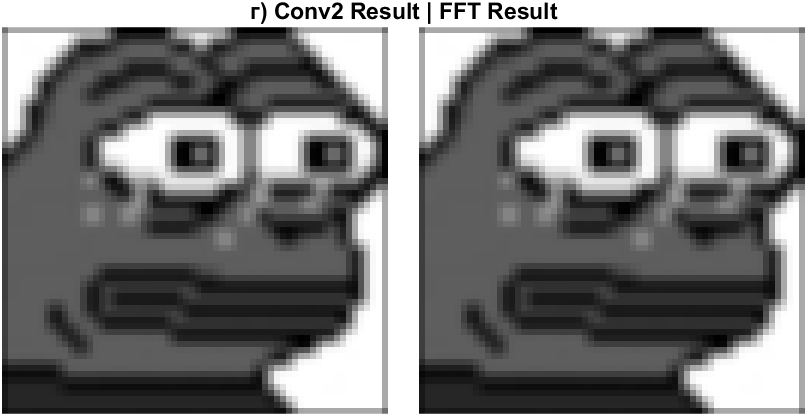
\includegraphics[width=0.8\textwidth]{б)/N=3/conv2_FFT.png}
    \caption{Сравнение результата свёртки и преобразования Фурье при $N=3$.}
\end{figure}



\paragraph*{Размытие при $N = 5$}
\hfill\\[5pt]

Ядро блочного размытия:
\begin{equation*}
K_{\sigma}^{(5)} = \frac{1}{25}\mathbf{1}_{5\times5} = \begin{bmatrix}
0.04 & 0.04 & 0.04 & 0.04 & 0.04 \\
0.04 & 0.04 & 0.04 & 0.04 & 0.04 \\
0.04 & 0.04 & 0.04 & 0.04 & 0.04 \\
0.04 & 0.04 & 0.04 & 0.04 & 0.04 \\
0.04 & 0.04 & 0.04 & 0.04 & 0.04
\end{bmatrix}
\end{equation*}
\begin{figure}[H]
    \centering
    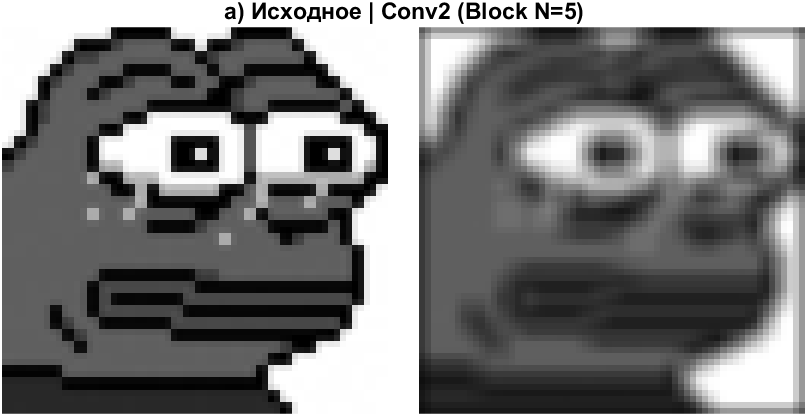
\includegraphics[width=0.8\textwidth]{б)/N=5/Orig_conv2.png}
    \caption{Слева - исходное чёрно-белое изображение, справа - результат свёртки с блочным ядром при $N=5$.}
\end{figure}
Изображение стало темнее, это говорит об увеличении эффекта при $N=5$ и явно видно как размылилась картинка с блочным ядром.

\begin{figure}[H]
    \centering
    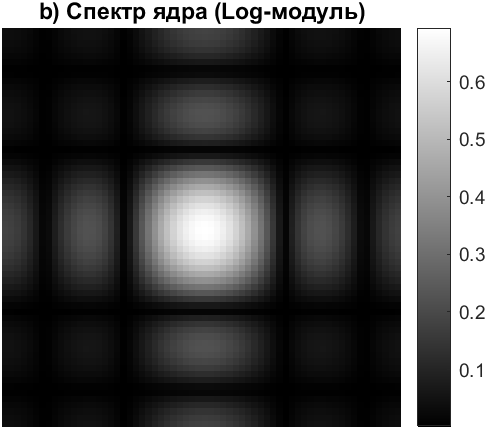
\includegraphics[width=0.8\textwidth]{б)/N=5/conv2_spektr.png}
    \caption{Спектр ядра блочного размытия при $N=5$.}
\end{figure}

\begin{figure}[H]
    \centering
    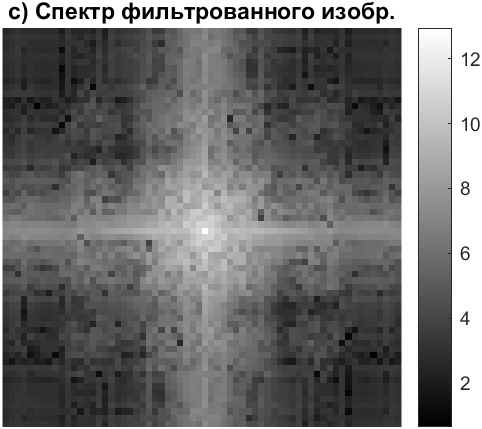
\includegraphics[width=0.8\textwidth]{б)/N=5/filt_spektr.png}
    \caption{Спектр фильтрованного изображения при $N=5$.}
\end{figure}

\begin{figure}[H]
    \centering
    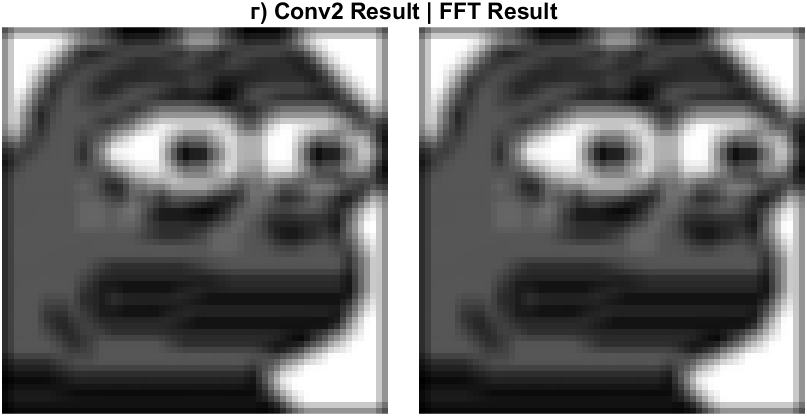
\includegraphics[width=0.8\textwidth]{б)/N=5/conv2_FFT.png}
    \caption{Сравнение результата свёртки и преобразования Фурье при $N=5$.}
\end{figure}
Результаты похожи, что подтвержает теорему о свертке.

\paragraph*{Размытие при $N = 7$}
\hfill\\[5pt]

Ядро блочного размытия:
\begin{equation*}
K_{\sigma}^{(7)} = \frac{1}{49}\mathbf{1}_{7\times7} \approx \begin{bmatrix}
0.0204 & \cdots & 0.0204 \\
\vdots & \ddots & \vdots \\
0.0204 & \cdots & 0.0204
\end{bmatrix}
\end{equation*}

\begin{figure}[H]
    \centering
    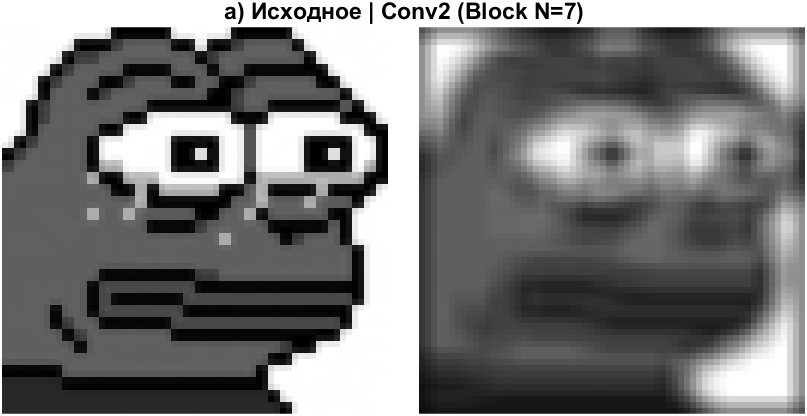
\includegraphics[width=0.8\textwidth]{б)/N=7/Orig_conv2.png}
    \caption{Слева - исходное чёрно-белое изображение, справа - результат свёртки с блочным ядром при $N=7$.}
\end{figure}

При использовании ядра блочного размытия размера $7 \times 7$ эффект сглаживания становится максимально выраженным. Изображение приобретает заметный «мыльный» эффект: мелкие детали и границы объектов практически исчезают. Поскольку все элементы ядра имеют одинаковый вес, фильтр сильно усредняет соседние пиксели, что приводит к потере резкости и контраста.


\begin{figure}[H]
    \centering
    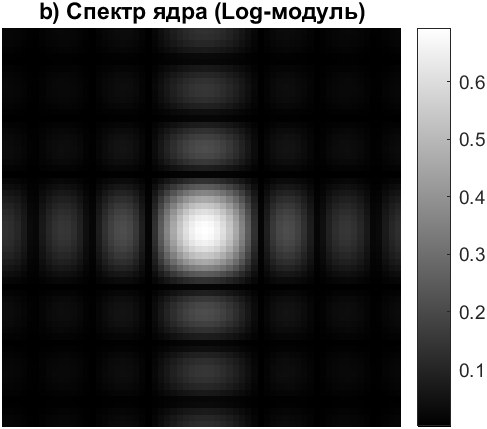
\includegraphics[width=0.8\textwidth]{б)/N=7/conv2_spektr.png}
    \caption{Спектр ядра блочного размытия при $N=7$.}
\end{figure}

\begin{figure}[H]
    \centering
    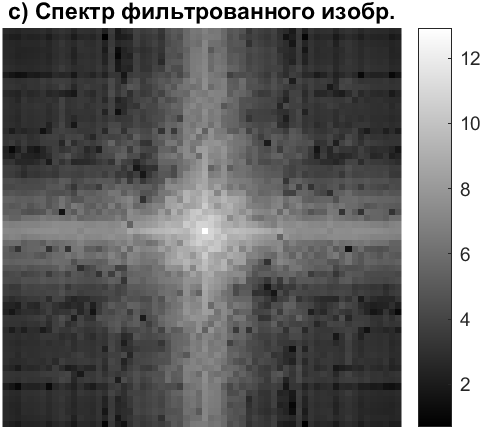
\includegraphics[width=0.8\textwidth]{б)/N=7/filt_spektr.png}
    \caption{Спектр фильтрованного изображения при $N=7$.}
\end{figure}

\begin{figure}[H]
    \centering
    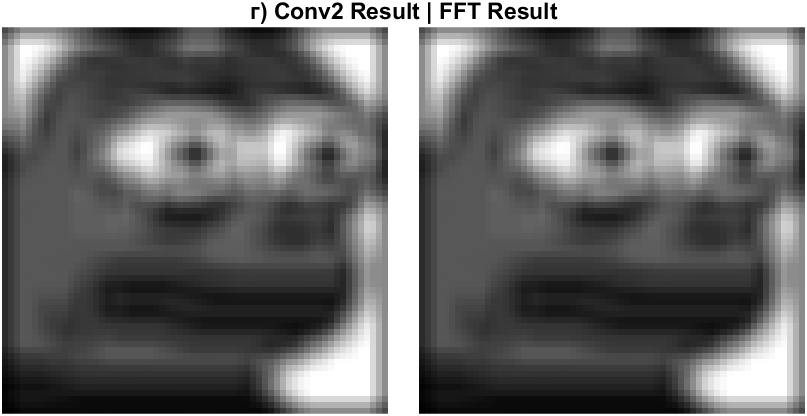
\includegraphics[width=0.8\textwidth]{б)/N=7/conv2_FFT.png}
    \caption{Сравнение результата свёртки и преобразования Фурье при $N=7$.}
\end{figure}

%==============================
\subsubsection*{в) Ядро увеличения резкости}

Ниже приведена матрица увеличения резкости и ее результат для нашего случая.

\begin{equation}
K_{*} = \begin{bmatrix}
0 & -1 & 0 \\
-1 & 5 & -1 \\
0 & -1 & 0
\end{bmatrix}.
\end{equation}

\begin{figure}[H]
    \centering
    
\includegraphics[width=0.8\textwidth]{в)/Orig_conv2.png}
    \caption{Слева - исходное чёрно-белое изображение, справа - результат свёртки с ядром увеличения резкости.}
\end{figure}



После применения фильтра увеличения резкости изображение становится более контрастным. Границы объектов усиливаются, а мелкие детали становятся более выраженными. В отличие от фильтров размытия, данный оператор подчёркивает перепады яркости.

\begin{figure}[H]
    \centering
    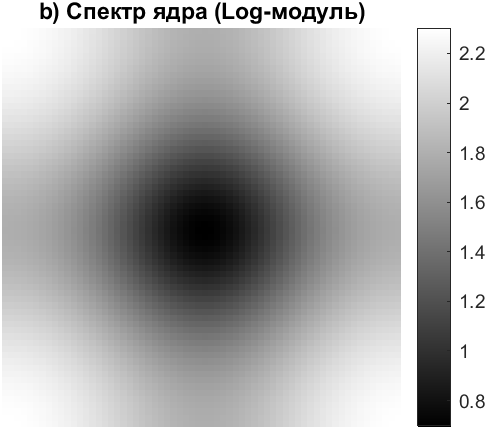
\includegraphics[width=0.8\textwidth]{в)/conv2_spektr.png}
    \caption{Спектр ядра увеличения резкости.}
\end{figure}
Спектр ядра показывает усиление высокочастотных компонент, что объясняет эффект повышения резкости и выделения мелких деталей изображения.

\begin{figure}[H]
    \centering
    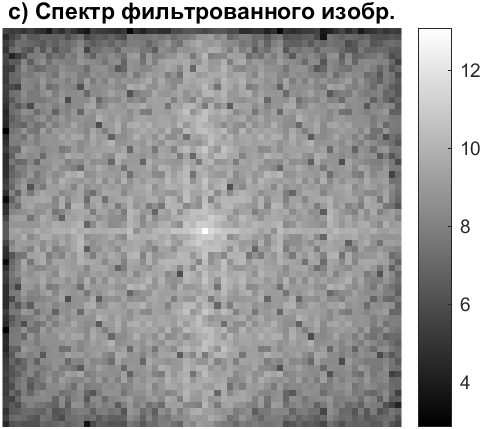
\includegraphics[width=0.8\textwidth]{в)/filt_spektr.png}
    \caption{Спектр обработанного изображения после применения фильтра резкости.}
\end{figure}
После фильтрации наблюдается перераспределение энергии спектра в сторону высоких частот, что соответствует усилению границ и текстурных элементов изображения.

\begin{figure}[H]
    \centering
    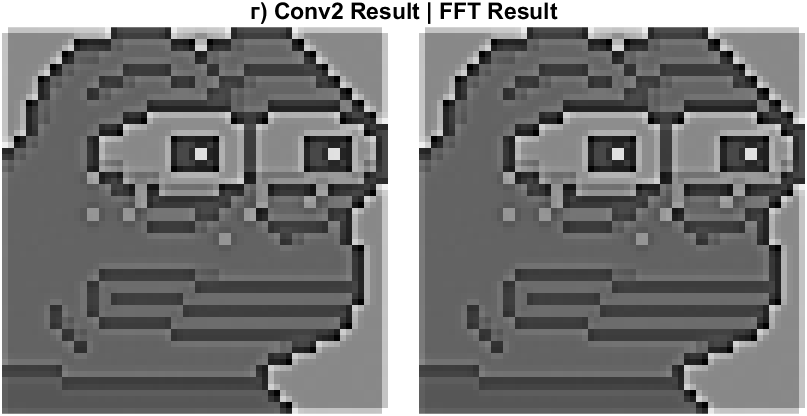
\includegraphics[width=0.8\textwidth]{в)/conv2_FFT.png}
    \caption{Сравнение результата свёртки и преобразования Фурье для фильтра увеличения резкости.}
\end{figure}
Результаты, полученные двумя способами (свёртка и преобразование Фурье), совпадают, что подтверждает корректность реализации теоремы о свёртке в дискретном случае.

\subsubsection*{г) Ядро выделения краев}

Ниже приведена матрица выделения краев и ее результат для нашего случая.

\begin{equation}
K_{\nabla} = \begin{bmatrix}
-1 & -1 & -1 \\
-1 & 8 & -1 \\
-1 & -1 & -1
\end{bmatrix}.
\end{equation}

\begin{figure}[H]
    \centering
    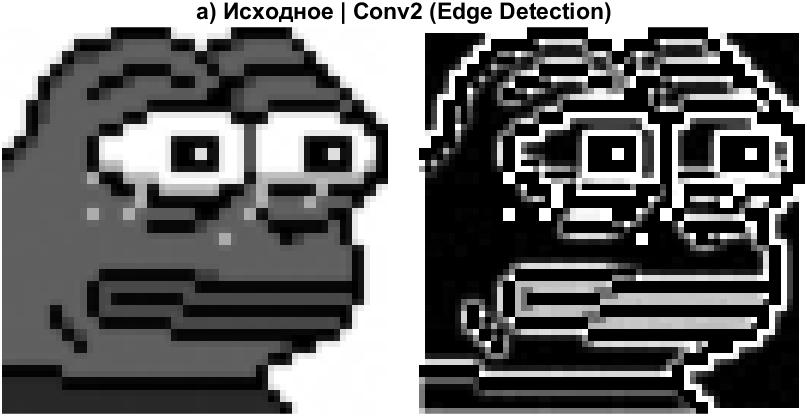
\includegraphics[width=0.8\textwidth]{г)/Orig_conv2.png}
    \caption{Слева - исходное чёрно-белое изображение, справа - результат свёртки с ядром выделения краёв.}
\end{figure}

\paragraph*{Анализ}

После применения данного фильтра становятся заметны границы объектов на изображении. Однородные области подавляются, а резкие перепады яркости, наоборот, усиливаются. В результате изображение приобретает характер «контурной карты», где выделены основные структурные элементы сцены.

\begin{figure}[H]
    \centering
    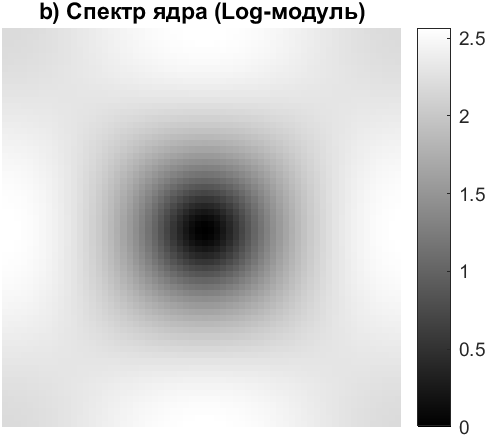
\includegraphics[width=0.8\textwidth]{г)/conv2_spektr.png}
    \caption{Спектр ядра выделения краёв.}
\end{figure}
Спектр ядра показывает усиление высокочастотных компонент, что соответствует его назначению — выделению резких изменений яркости и контуров изображения.

\begin{figure}[H]
    \centering
    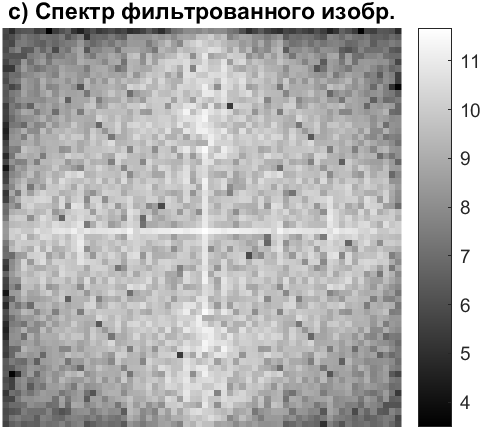
\includegraphics[width=0.8\textwidth]{г)/filt_spektr.png}
    \caption{Спектр обработанного изображения после применения фильтра выделения краёв.}
\end{figure}
После фильтрации наблюдается усиление высокочастотных составляющих, соответствующих границам объектов. Низкочастотные области подавляются, поэтому изображение приобретает контурный характер.

\begin{figure}[H]
    \centering
    
\includegraphics[width=0.8\textwidth]{г)/conv2_FFT.png}
    \caption{Сравнение результата свёртки и преобразования Фурье для фильтра выделения краёв.}
\end{figure}
Результаты, полученные двумя методами (свёрткой и через преобразование Фурье), совпадают с высокой точностью, что подтверждает корректность реализации теоремы о свёртке в дискретном случае.


\subsection*{Сравнение методов}

\begin{table}[H]
\centering
\caption{Сравнение максимальной разницы между методами свёртки}
\begin{tabular}{|l|c|}
\hline
\textbf{Ядро} & \textbf{Max разница} \\
\hline
Gaussian N=3 & $\approx 0$ \\
Box N=5 & $\approx 0$ \\
Edge Detection & $\approx 0$ \\
\hline
\end{tabular}
\end{table}

Различия между результатами свёртки через \texttt{conv2} и через FFT близки к 0 (численная погрешность), что подтверждает выполнение \textbf{теоремы о свёртке}.



\subsection*{Вывод по заданию}

В ходе работы были исследованы различные типы ядер свёртки и их влияние на изображение в пространственной и частотной областях. Для обработки использовались гауссовы и блочные фильтры размытия с размерами $N=3$, $N=5$ и $N=7$, а также ядро увеличения резкости и ядро выделения краёв.

Было установлено, что при увеличении размера ядра размытия эффект сглаживания усиливается. Гауссов фильтр обеспечивает более естественное размытие за счёт большего веса центральных элементов ядра, тогда как блочное размытие приводит к сильному усреднению пикселей и появлению «мыльного» эффекта. Фильтр увеличения резкости, наоборот, усиливает высокочастотные компоненты изображения, делая границы объектов и мелкие детали более выраженными. Ядро выделения краёв подавляет однородные области и позволяет выделить контуры изображения.

Также были исследованы спектры ядер и обработанных изображений с использованием дискретного преобразования Фурье. Анализ спектров показал, что фильтры размытия подавляют высокочастотные составляющие, а фильтры резкости и выделения краёв усиливают их.

В работе была экспериментально подтверждена теорема о свёртке: результат свёртки изображения в пространственной области совпадает с результатом, полученным через поэлементное умножение спектров в частотной области с последующим обратным преобразованием Фурье. Незначительные различия между изображениями связаны с особенностями дискретизации, округления и обработки границ.

Таким образом, были изучены основные методы линейной фильтрации изображений, а также исследована связь между пространственным и частотным представлением изображений.
% \begin{enumerate}
%     \item \textbf{Эквивалентность методов}: Пространственная свёртка (\texttt{conv2}) и частотная свёртка (через FFT) дают идентичные результаты (с точностью до машинной погрешности), что подтверждает теорему о свёртке.
    
%     \item \textbf{Эффективность FFT}: Для больших ядер преобразование Фурье может быть вычислительно более эффективным, так как сложность FFT составляет $O(n \log n)$ против $O(n^2)$ для прямой свёртки.
    
%     \item \textbf{Визуализация в частотной области}: Логарифм модуля Фурье-образа позволяет наглядно увидеть частотные характеристики изображения и фильтров.
    
%     \item \textbf{Эффекты ядер}:
%     \begin{itemize}
%         \item Гауссово и блочное размытие подавляют высокие частоты (низкочастотные фильтры)
%         \item Ядро резкости и выделения краёв подчёркивают высокие частоты (высокочастотные фильтры)
%     \end{itemize}
    
%     \item \textbf{Zero padding}: Дополнение нулями необходимо для получения линейной (не циклической) свёртки и корректного применения теоремы о свёртке.
% \end{enumerate}

\section*{Вывод}

В ходе лабораторной работы было рассмотрено применение двумерного преобразования Фурье к обработке изображений. В первом задании было показано, что периодические искажения удобно удалять в частотной области, так как они проявляются в виде отдельных пиков на Фурье-образе. Подавление этих пиков позволило ослабить помеху и сохранить основное содержание изображения.

Во втором задании были исследованы разные ядра свёртки. Было показано, что фильтры размытия подавляют высокочастотные компоненты изображения, а фильтры резкости и выделения краёв, наоборот, усиливают их. Также было подтверждено, что свёртка в пространственной области эквивалентна умножению спектров в частотной области.

Таким образом, работа показала, что частотное представление изображения позволяет наглядно анализировать действие фильтров и выполнять обработку изображений.

\end{document}